\documentclass[11pt,a4paper]{article}
% --- transparent修补 ---
\makeatletter
\@ifpackageloaded{transparent}{}{
    \providecommand{\IfPDFManagementActiveF}[2]{#2}
}
\makeatother

\usepackage[UTF8]{ctex}
\usepackage{geometry}
\usepackage{graphicx}
\usepackage{float}
\usepackage{amsmath}
\usepackage{amssymb}
\usepackage{booktabs}
\usepackage{multirow}
\usepackage{hyperref}
\usepackage{caption}
\usepackage{subcaption}
\usepackage{listings}
\usepackage{xcolor}
\usepackage{tikz}
\usepackage{pgfplots}
\pgfplotsset{compat=1.18}   % 添加这个以消除 pgfplots 警告
\usetikzlibrary{positioning, arrows.meta, shapes.geometric} % 关键

\usepackage{svg}
\usepackage{url}
\usepackage{bm}
% 如果您不需要 mermaid 可以注释掉下一行
\usepackage{mermaid} 

\geometry{left=2.5cm, right=2.5cm, top=2.5cm, bottom=2.5cm}

\title{\textbf{基于视觉基元的思维：迈向高效多模态推理}}
\author{DeepSeek-AI$^1$，北京大学$^2$，清华大学$^3$ \\ $^1$核心贡献者 $^2$项目负责人}
\date{2026年5月}

\begin{document}

\maketitle

\begin{abstract}
尽管多模态大语言模型（MLLMs）取得了显著进展，但主流的思维链（CoT）范式仍主要局限在语言空间。近期的研究虽然通过高分辨率裁剪（如“基于图像的思维”）来弥合感知鸿沟，却忽略了更根本的瓶颈：指代鸿沟。自然语言固有的歧义性往往无法为复杂的空间布局提供精确、无歧义的指引，导致在需要严格定位的任务中出现逻辑崩溃。本文提出一种全新的推理框架——\textbf{基于视觉基元的思维}（Thinking with Visual Primitives），将空间标记（如点和边界框）提升为“思维的最小单元”。通过将这些视觉基元直接交织到思维过程中，我们的模型能够“边指点边推理”，从而将认知轨迹有效锚定在图像的物理坐标上。值得注意的是，我们的框架基于高度优化的架构，具有极致的视觉令牌效率。尽管模型规模紧凑且图像令牌预算显著更低，我们的模型在一系列具有挑战性的视觉问答任务上仍达到了前沿水平，匹配甚至超越了GPT-5.4、Claude-Sonnet-4.6和Gemini-3-Flash等模型。这展示了一条通往更高效、可扩展的类系统2多模态智能的路径。
\end{abstract}

\section{引言}

大语言模型与计算机视觉的融合催生了能够进行复杂场景理解的多模态大语言模型（MLLMs）。然而，当我们推动这些模型进行复杂推理（通常被概念化为丹尼尔·卡尼曼的“系统2”思维[23]）时，当前范式的一个根本局限性逐渐显现。虽然这些模型的内部推理（通常表现为思维链）在语言领域已变得日益稳健，但其与视觉领域在很大程度上仍然是脱节的。

近期增强多模态推理的努力，例如前沿模型中的视觉规模化策略[8,12,21,24,26,34]，主要解决了\textbf{感知鸿沟}。通过采用高分辨率裁剪和动态分块，这些模型确保了它们能“看见”图像中的细粒度细节。然而，“看见”不等于“推理”。即使具备完美的感知能力，MLLMs在涉及复杂空间布局或密集物体交互的任务中仍然经常遭受逻辑崩溃。我们将这种失败识别为\textbf{指代鸿沟}：自然语言在连续的视觉空间中作为精确、无歧义指针的固有能力缺失。在密集计数或多步空间演绎等场景中，模型的语言“思维”会丢失它们意图指代的视觉实体，导致级联幻觉。虽然近期工作[6,27,32]探索了将边界框集成到思维链过程中，但它们主要将定位视为一种事后验证机制，用于增强感知密集型任务。这些方法通常局限于“看见”而非“推理”成为挑战的高分辨率基准，并且它们对大量人工标注的依赖限制了可扩展性。更重要的是，它们未能解决复杂结构推理（如拓扑导航）中的指代鸿沟，在那里视觉标记必须作为思维的内在媒介，而不仅仅是可验证的证据。

在本文中，我们提出一个范式转变：\textbf{基于视觉基元的思维}。我们不再将视觉定位视为辅助任务或最终输出，而是将空间标记——点和边界框——提升为“思维的最小单元”，并直接交织到模型的推理轨迹中。这一机制汲取了人类认知过程的灵感。当人类在复杂迷宫中导航或计数密集物体时，会自然地使用指示性指针（例如手指动作）来降低认知负荷并保持逻辑一致性。通过将视觉基元交织到思维过程中，我们的模型模仿了这种“指点-推理”协同效应，有效地将抽象的语言思想锚定在具体的空间坐标上。

此外，我们的框架建立在架构高效的基础之上[3]，专为高吞吐量、长上下文的多模态交互而设计。与依赖海量视觉令牌序列来弥补视觉缺陷的传统方法不同，我们的模型利用\textbf{压缩稀疏注意力（CSA）}[3]，将每$m$个视觉令牌的键值（KV）缓存压缩为一个条目。这种设计使得模型仅需使用其他前沿系统一小部分的视觉令牌，就能保持相当的认知深度。

通过广泛的基准测试，我们证明了“基于视觉基元的思维”在推理准确性上带来了显著的飞跃。我们的模型在广泛的有挑战性的空间推理和视觉问答任务上取得了与GPT、Claude和Gemini最新版本相当甚至更优的性能（见图1）。我们的发现表明，多模态智能的未来不仅在于看到更多的像素，更在于开发更精确、更少歧义的指代机制，从而弥合语言与视觉世界之间的鸿沟。

\begin{figure}[H]
\centering
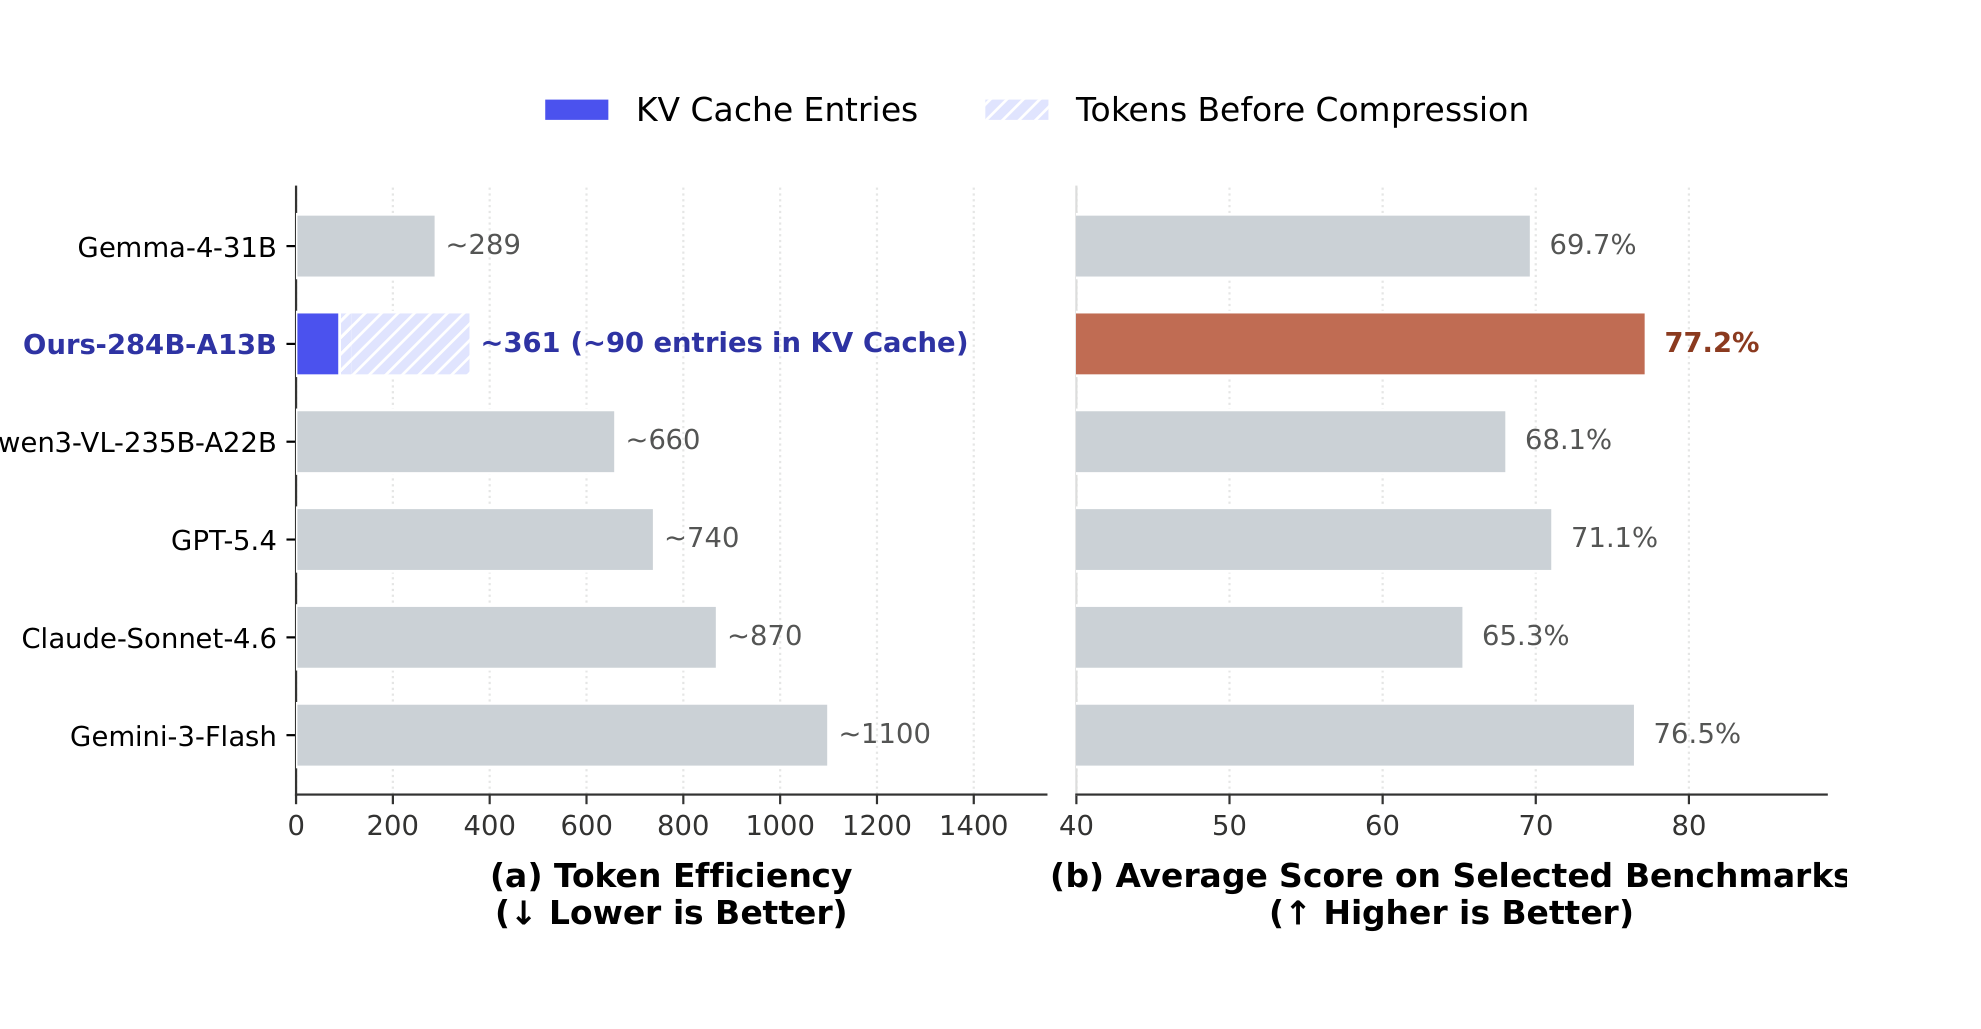
\includegraphics[width=\textwidth]{../figures/Thinking_with_Visual_Primitives_fig01.png}
\caption{（a）各模型在$800\times800$分辨率图像上的令牌消耗。（b）7个基准（包括计数和空间推理）的平均性能。我们的模型仅保留约90个KV缓存条目，通过高效的压缩策略实现竞争性性能。}
\label{fig:token}
\end{figure}

\section{方法}

\subsection{概述}

本节首先介绍模型架构，然后详细阐述训练流水线（如图2所示），并描述预训练和后训练阶段使用的相应数据。

\subsection{架构}

我们的模型采用类似于LLaVA[18,19]的标准架构。具体来说，输入图像由视觉Transformer（ViT）处理以提取视觉特征，然后与语言指令拼接形成交织的视觉-语言令牌序列。该序列随后被输入到大语言模型（LLM）以生成响应。语言骨干采用\textbf{DeepSeek-V4-Flash}[3]，这是一个混合专家（MoE）模型，总计284B参数，推理时激活13B参数。

对于视觉编码，我们使用内部从头训练的\textbf{DeepSeek-ViT}，它支持任意分辨率输入。首先使用$14\times14$的块大小对输入图像进行分块生成块令牌。随后，在ViT输出处，我们应用$3\times3$空间令牌压缩（将每9个相邻的块令牌沿通道维度压缩为一个令牌）。此外，利用基础LLM中集成的\textbf{压缩稀疏注意力（CSA）}机制，KV缓存中的视觉令牌被进一步压缩4倍。

以$756\times756$分辨率的输入图像为例，包含571,536像素。分块嵌入层生成2,916个图像块令牌供ViT使用。经过$3\times3$压缩后，只有324个视觉令牌在预填充阶段被送入LLM。最终，CSA机制将其减少到仅仅81个视觉KV缓存条目。从原始像素到最终KV缓存条目，整个系统实现了\textbf{7,056倍}的总体压缩比。

\begin{figure}[H]
\centering
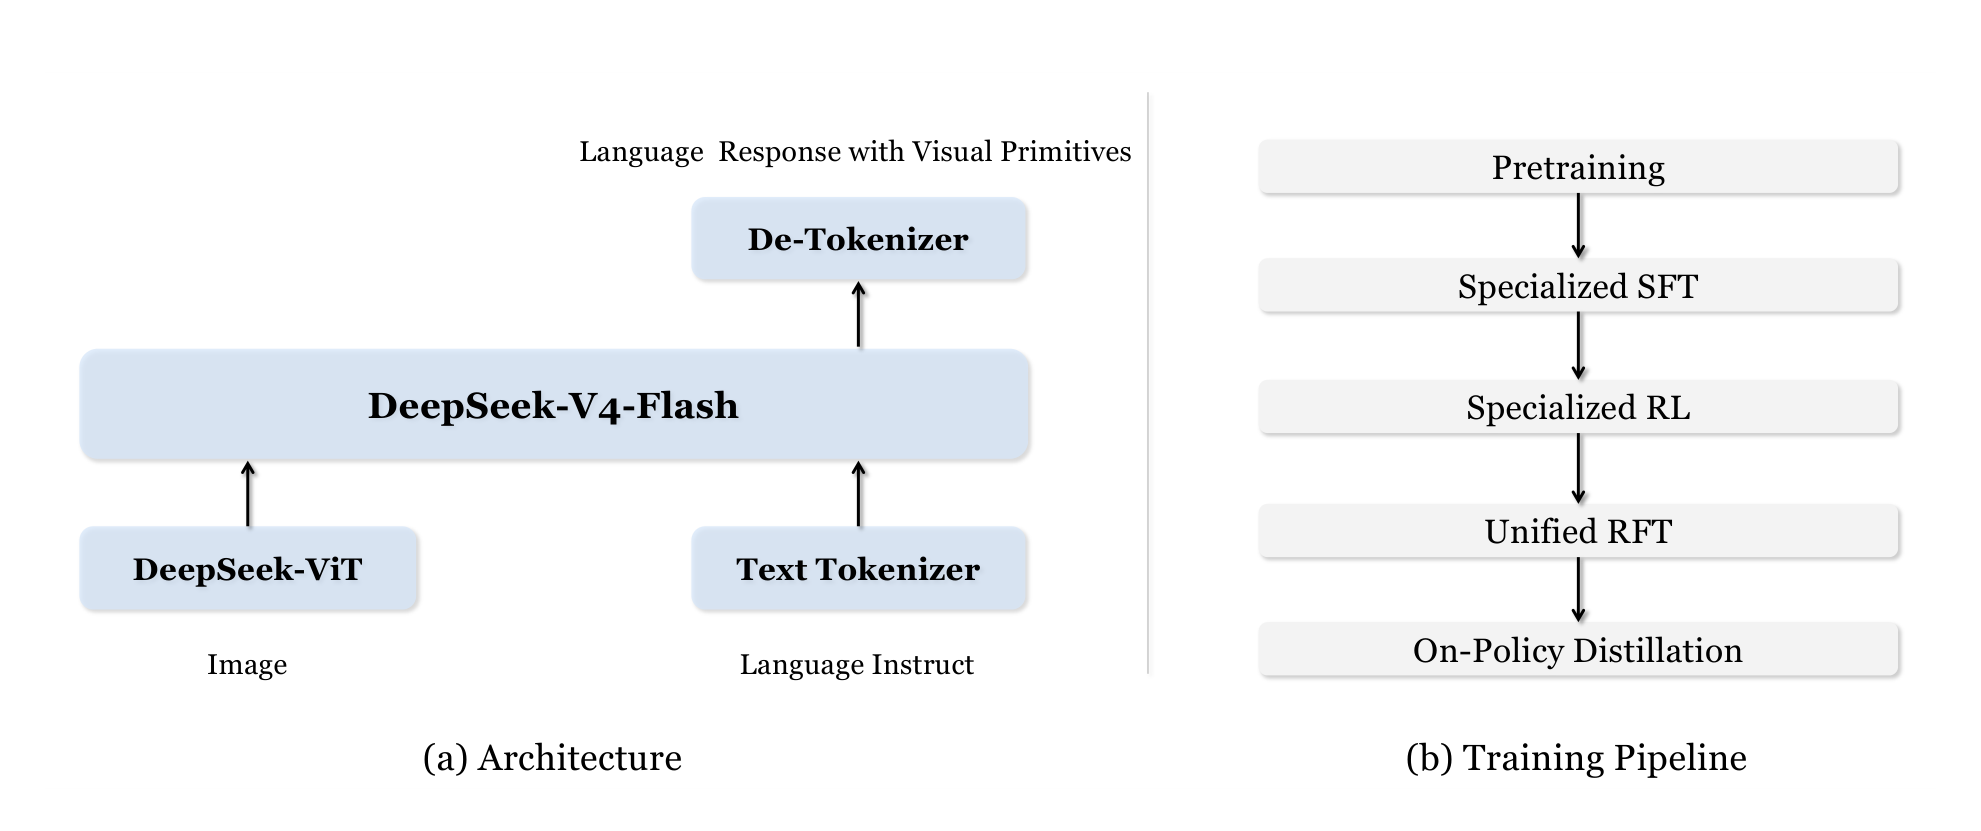
\includegraphics[width=\textwidth]{../figures/Thinking_with_Visual_Primitives_fig02.png}
\caption{模型架构与训练流水线。预训练阶段获得基础的视觉基元生成能力，随后进行后训练，采用专家式专门化与整合范式。}
\label{fig:arch}
\end{figure}

\subsection{预训练}

\subsubsection{视觉基元的定义}

预训练阶段的目标是使模型具备输出“视觉基元”的基本能力。我们确定计算机视觉中的两种标准输出格式作为基元：边界框和点。这两种表示都承担着空间引用的关键角色。然而，它们具有不同的功能优势：边界框擅长捕捉特定物体的精确位置和尺度，而点更适用于抽象视觉引用，如跟踪运动轨迹或解决拓扑推理问题。

\subsubsection{大规模数据整理的动机}

虽然现有的公共数据集（如COCO[17]和Pixmo-Points[4]）提供了相对准确的框或点标注，但它们规模不足且多样性欠缺。为确保“基于视觉基元的思维”范式的泛化能力，必须整理具有丰富语义和高多样性的大规模网络数据。我们优先扩展边界框数据的规模，原因如下：

\begin{itemize}
    \item \textbf{标注确定性}：边界框紧密包围物体，其标注相对确定。相反，点标注高度模糊；物体边界内的任何坐标都可作为有效参考，导致缺乏严格的真值。在极端遮挡场景下，指向背景物体的点可能落在前景遮挡物上，造成显著歧义。
    \item \textbf{任务泛化性}：经边界框训练的模型可以轻松泛化到基于点的格式。由于边界框可以由两个点（左上和右下坐标）定义，它天然包含点表示。
    \item \textbf{信息丰富性}：与点相比，边界框支持更广泛的下游任务。点仅提供空间定位，而边界框封装了详细的几何信息（如宽度和高度）。这种额外的上下文使模型能够在“基于视觉基元的思维”框架内执行更复杂的推理。
\end{itemize}

\subsubsection{大规模网络数据构建}

\textbf{原始数据获取}。我们通过大规模网页抓取获取与框定位相关的海量互联网数据。以Huggingface为例，利用其官方API过滤标记为“Object Detection”或“Grounding”的任务数据。基于流行度指标（如下载量和点赞数）进行初步筛选，并严格排除所有验证集和测试集以防止评估时的数据污染。此外，我们使用基于LLM的代理解析这些仓库的README.md文件，自动将各种数据集结构转换为预定义的统一存储格式。经过广泛的爬取和去重，最终整理出97,984个框定位相关数据源。对采样数据的人工检查显示物体类别高度多样，涵盖从常见目标（如人、脸）到领域特定实体（如CT扫描中的病变区域或特定动漫角色）。然而，这些原始框标注仍然存在各种问题，如语义模糊和几何不准确，需要进一步严格过滤。我们设计了两步过滤流水线，如下所示。

\textbf{第一步：基于语义的审查}。由于直接爬取的数据集包含大量不适合视觉-语言对齐训练的噪声标签，我们引入自动化的MLLM驱动的语义审查机制。传统数据过滤主要关注边界框的几何准确性，而此阶段旨在确保语义标签的有效性。具体来说，该审查过程专注于消除三类致命的语义缺陷：

\begin{itemize}
    \item \textbf{无意义的机器代码和无意义文本}：许多原始数据集保留内部开发代码（如纯数字类“0”或“1”）。由于这些标签缺乏人类可读的自然语言语义，强迫模型学习这种映射会严重损害其语言生成能力，因此直接丢弃。
    \item \textbf{无法泛化的私有实体}：某些数据集使用特定的人称代词（如“MyRoommate”）或私有标识符（如“ID\_Card\_1”）。由于MLLM无法从孤立样本中泛化非公众人物的视觉特征（即“某人”的视觉特征无法泛化到通用概念），这类数据被严格过滤掉。相反，广泛认可的名人或公众人物则保留。
    \item \textbf{模糊的缩写和主观评价}：特定领域（如工业检测）中常见的标签，如“OK”或“NG”（Not Good），通常缺乏具体的视觉描述性。例如，一个简单的“OK”标签引入了极端的语义模糊性，因为“完整的苹果”和“完整的电路板”没有任何视觉相关性。
\end{itemize}

对于每个数据集，我们采样三张图像，并提示模型根据上述标准计算质量分数（0-10）。模型输出明确的“KEEP”或“DISCARD”决定，并附有清晰的理由。此审查阶段保留了43,141个数据源（初始为97,984个），进入下一过滤阶段。

\textbf{第二步：视觉-几何质量审查}。我们进一步评估边界框的几何质量和标注完整性，以确保模型学习精确的区域-文本对齐。此过程专门针对三种类型结构标注缺陷：

\begin{itemize}
    \item \textbf{严重漏标（低召回）}：指图像中存在多个与给定标签对应的实例，但只有少数被标注。如果采样时检测到大面积漏标（如漏标率>50\%），则该数据集立即丢弃。
    \item \textbf{严重截断和偏移}：指边界框未能合理包含目标物体。实际中我们采用差异容忍策略：略微宽松的框（包含少量背景噪声）被认为是可接受的；但严重截断物体关键视觉特征（如切断头部或车轮）的框严格不可接受。
    \item \textbf{巨型框问题}：如果边界框无意义地覆盖超过90\%的图像面积，通常表明图像分类数据被强制转换为检测数据。如果这仅偶尔出现在采样批次中，则视为可接受的噪声。但如果这种全局框在所有三张采样图像中持续出现，则认为该数据集缺乏有意义的定位信息，予以丢弃。
\end{itemize}

此审查阶段进一步保留了31,701个数据源（从43,141个）。为实现数据集平衡，我们设计了一种基于类别的采样策略。对于每个数据集中每个类别，我们随机采样$N$张与该类别相关的图像（如果该类别可用图像总数少于$N$，则全部保留）。由于单张图像可能同时属于多个类别，我们在每类别选择后对汇总集进行全局去重。实践中设置$N=1,000$，最终获得超过4000万个高质量样本。

\subsubsection{统一预训练}

对于通用多模态数据，我们主要使用大规模网络爬取的数据，而不是通过模型蒸馏生成的合成数据（如合成图像描述）。原始数据经过仔细整理，我们避免使用LLM重写数据内容。对于专门用于赋予模型输出视觉基元基础能力的数据，除了上述网络爬取和过滤外，我们还整合了几个高质量的公共数据集，如[4,15,17,25,29,33]。我们为框定位和点数据建立统一的格式标准。对于框定位任务，我们设计了几种提示模板，例如“在图像中找到TARGET并报告其边界框坐标。”其中TARGET为查询物体的占位符。对应的响应格式为：\texttt{<|ref|>TARGET</|ref|><|box|>[[x1,y1,x2,y2], [x3,y3, x4,y4]...]<|/box|>}，其中\texttt{<|ref|>}、\texttt{</|ref|>}、\texttt{<|box|>}和\texttt{</|box|>}是词汇表中的特殊标记。$x1,y1$和$x2,y2$表示边界框的左上和右下坐标，归一化为0到999之间的离散整数。对于多实例场景，边界框从左到右排列。类似地，对于点任务，我们设计提示模板如“帮我找到TARGET。给出每个实例的中心点。”期望的响应格式为：\texttt{<|point|>[[x1,y1], [x2,y2]...]<|/point|>}，其中\texttt{<|point|>}和\texttt{</|point|>}是特殊标记，$x1,y1$表示点坐标。值得注意的是，与框定位格式不同，点任务的响应范式不需要输出物体名称。这一设计选择旨在将基于点的表示扩展到更抽象的概念，如利用一系列点来表示轨迹。最终，整个预训练阶段消耗了数万亿多模态令牌。

\subsection{任务设计与冷启动数据}

\subsubsection{冷启动数据}

虽然预训练赋予了模型通用的多模态先验和基本的视觉基元能力，但后训练（专门的SFT/RL及随后的统一RFT）需要一个小型但高精度的冷启动数据集，以在视觉基元输出接口下引导指令遵循和奖励学习。具体而言，我们构建的冷启动数据具有：(i) 来自标注（如框/点）或程序化生成的显式监督目标；(ii) 尽可能采用自动验证器（如基于规则的检查器）以减少标签噪声。我们选择了受益于视觉基元推理（通过框或点）的代表性任务，并在四个关键维度上设计冷启动数据：计数、空间推理与通用视觉问答、迷宫导航和路径追踪。

\paragraph{计数}
多模态大语言模型在准确计数方面持续挣扎，尤其是在密集场景中。与人类通常采用系统性扫描-累积策略不同，基于语言的模型在物体数量较多时往往无法建立精确的物体对应关系。我们通过采用边界框作为视觉基元来提供明确的指代锚点，以此解决这一根本瓶颈。

\textbf{任务分解。} 我们将计数任务分为两类：粗粒度计数和细粒度计数。前者侧重于对通用类别进行计数（如“狗”），后者要求基于特定属性或空间约束区分物体（如“白色的狗”或“左边的狗”）。

\textbf{粗粒度计数。} 我们从多个密集检测数据集中聚合数据，包括[2,9,14,22,28,29,35]。为确保数据质量，我们基于三个主要标准实施过滤：避免过度的物体密度、确保边界框足够大以便清晰识别、以及保持真值框标注的高召回率。对于过滤后的样本，我们提示MLLM基于图像和框标注生成思维内容和简洁的最终响应。思维内容生成遵循结构化的三步协议：(1) 意图分析，模型识别目标类别；(2) 批量定位，模型利用视觉基元同时定位所有候选物体（我们发现批量定位对于粗粒度任务更高效，因为它利用模型固有的定位能力同时避免重复枚举）；(3) 基于视觉基元的统计求和。为消除冷启动训练中的噪声，我们实施严格的验证机制，确保思维内容中的所有框视觉基元与元数据坐标严格对齐，遵循预定义语法，并与最终数值计数匹配。

\textbf{细粒度计数。} 由于公开数据集中缺乏专门用于细粒度计数的数据，我们开发了专门的数据构建流水线。(1) 问题生成：利用GQA[10]中的图像和场景图元数据，我们提示MLLM生成信息丰富的细粒度计数问题。无法产生有意义问题的样本被丢弃。对于每个有效样本，我们记录真值物体ID、被排除的负候选ID以及QA对构建的潜在理由。(2) 思维内容合成：使用图像、场景图和之前生成的问题（及其关联ID和理由）作为输入，我们引导MLLM合成与视觉基元交织的推理链。虽然整体思维结构类似于粗粒度计数，但模型被明确指示执行顺序扫描——系统性地识别和验证场景中每个可能的物体是否符合指定的细粒度约束。我们还应用此方法构建真值计数为零的负样本，从而增强模型抵抗幻觉的鲁棒性。

总计，我们为计数任务构建了约10,000个冷启动样本。示例如图3所示。

\begin{figure}[H]
\centering
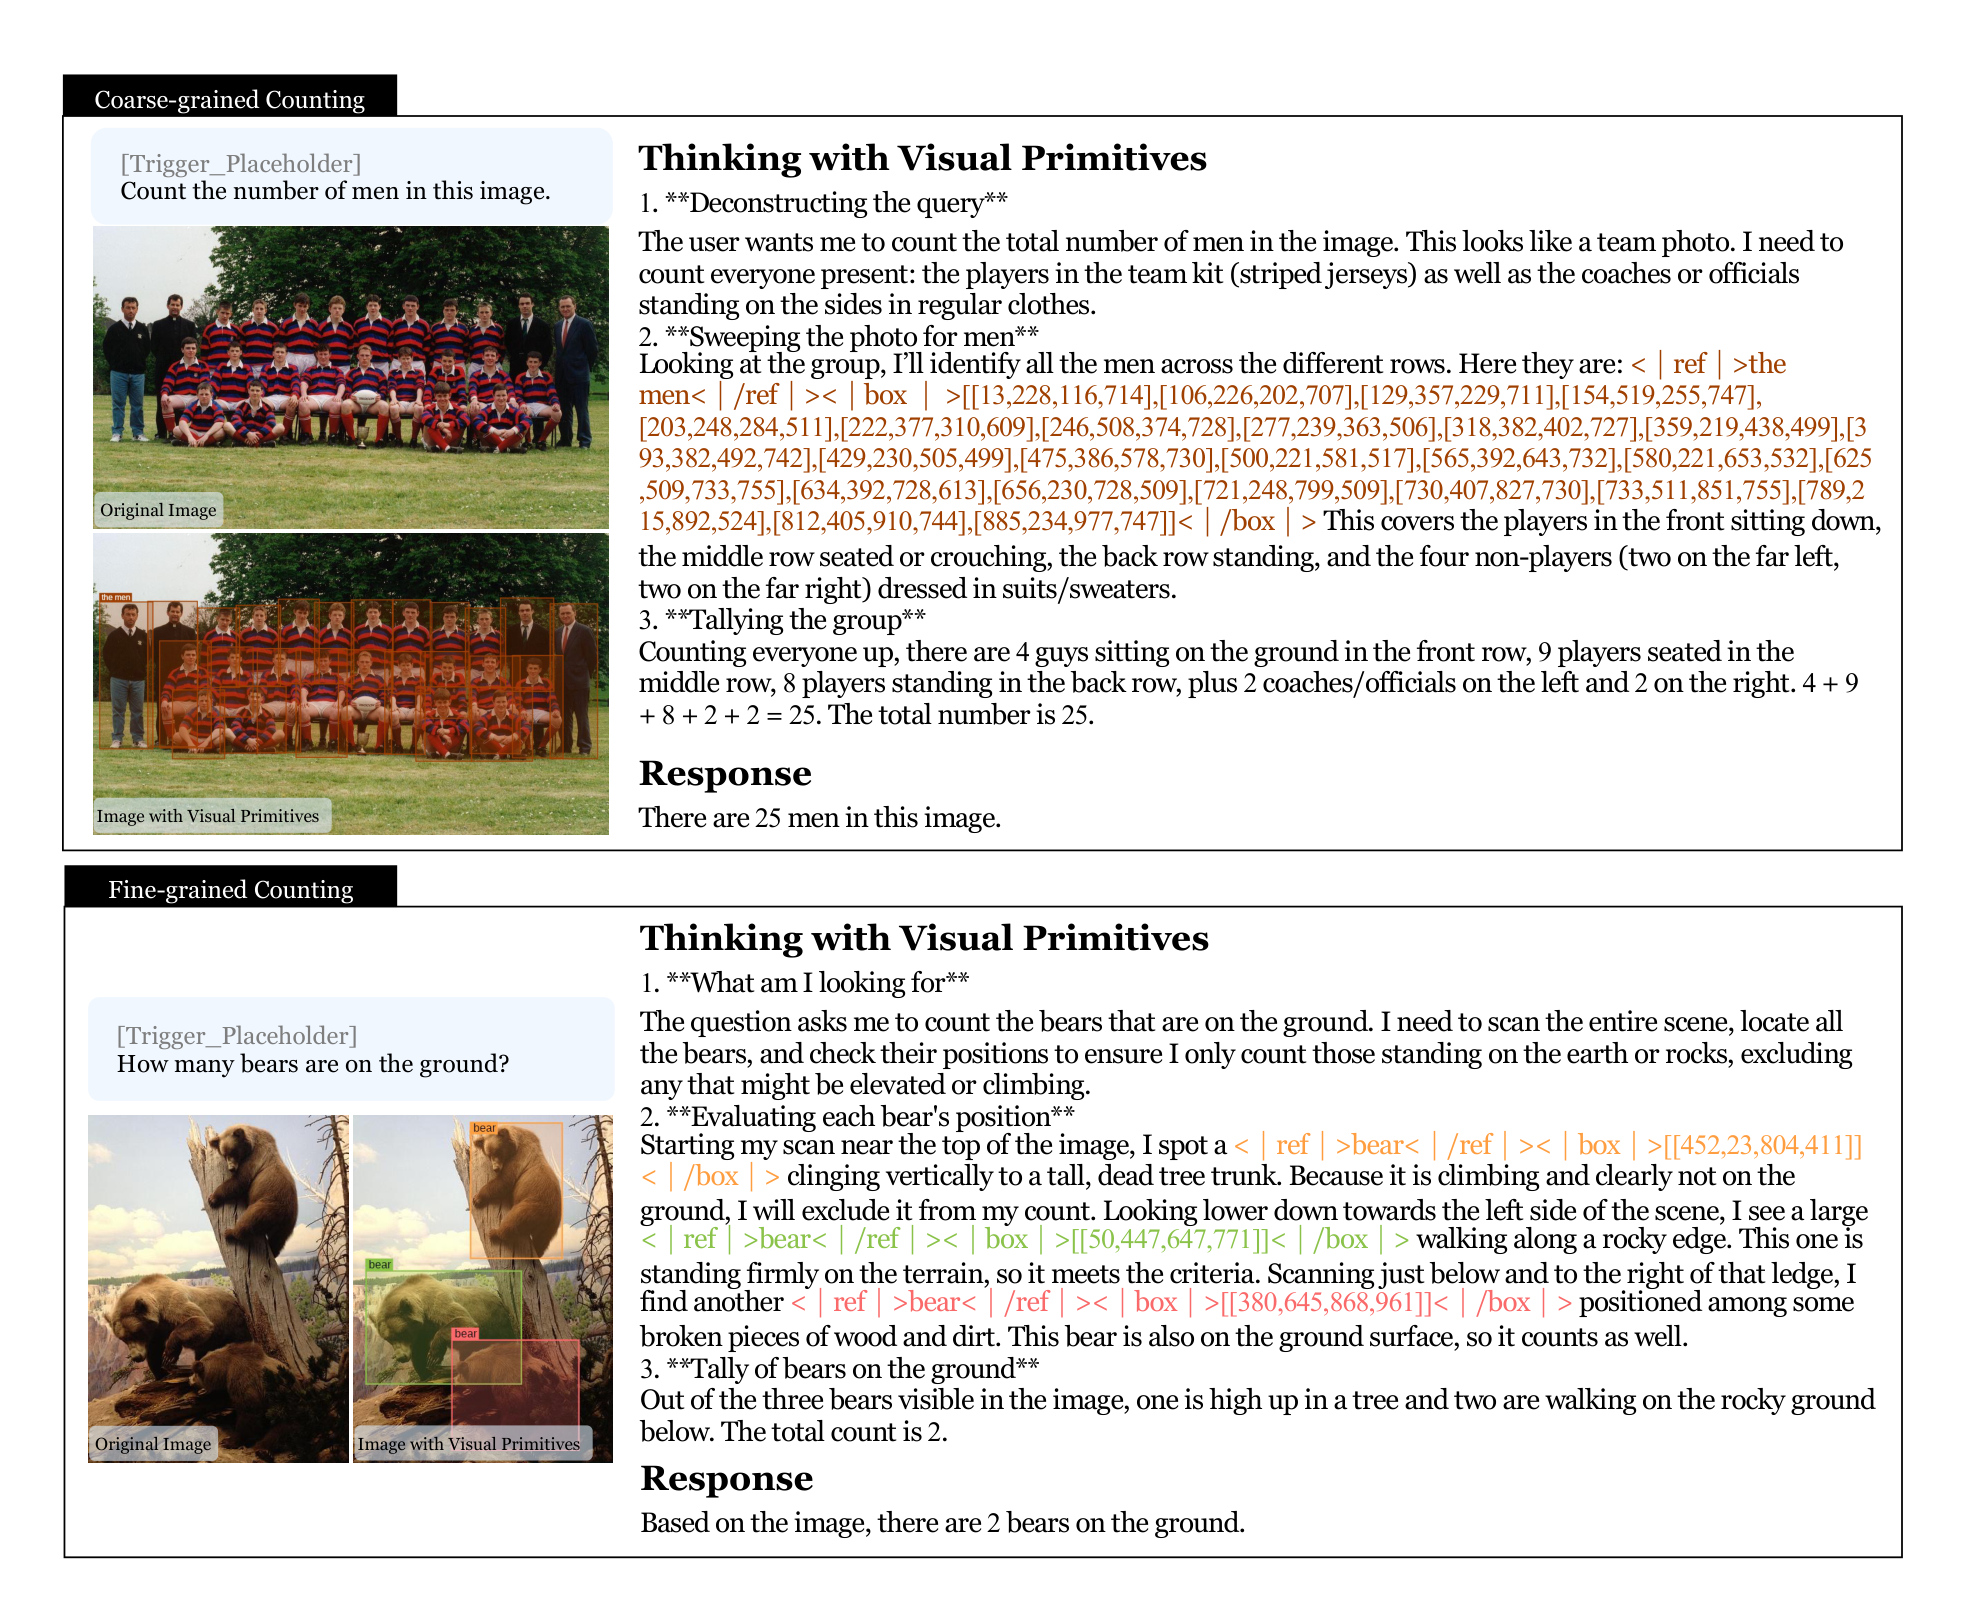
\includegraphics[width=\textwidth]{../figures/Thinking_with_Visual_Primitives_fig03.png}
\caption{计数任务的冷启动数据示例。模型进行意图分解并利用视觉基元锚定相关实体，随后进行系统性的计数过程。}
\label{fig:counting}
\end{figure}

\paragraph{空间推理与通用视觉QA}
我们将空间推理和通用VQA整合为一个统一类别。这种整合有效地缓解了纯语言描述中的指代模糊和语义漂移。在构建冷启动数据时，我们优先考虑空间推理任务，假设此处开发的“基于视觉基元的思维”能力将自然泛化到更广泛的VQA场景。我们的数据整理涵盖自然场景和合成场景。

\textbf{自然场景数据构建。} 利用GQA[10]中的图像和场景图，我们提示MLLM设计围绕空间关系和物体交互的问题以及相应的思维内容。生成的思维内容遵循结构化过程，包括意图分析、物体定位和关系推理。为解决拥挤场景中的潜在歧义，模型被指示选择独特物体并应用多属性约束（如结合动作和属性）来唯一指定目标。然而，由于GQA中相对简单的关系结构，难以大规模生成复杂的多跳推理样本。为克服这一限制并充分释放模型潜力，我们进一步整合了复杂的合成数据。

\textbf{合成场景数据构建。} 我们利用CLEVR[13]工具链生成多跳推理数据。该框架支持可控的场景生成（具有可变物体密度），以及问题生成和程序化执行跟踪，将每个推理步骤映射到物体级引用（如特定物体ID）。为监督视觉基元的生成，我们基于官方工具链将3D物体坐标投影到2D边界框。基于渲染的图像、场景图、问题、答案和执行跟踪，我们提示MLLM合成“基于视觉基元的思维”链，包括意图分析、任务分解和多跳定位推理。示例如图4所示。

\begin{figure}[H]
\centering
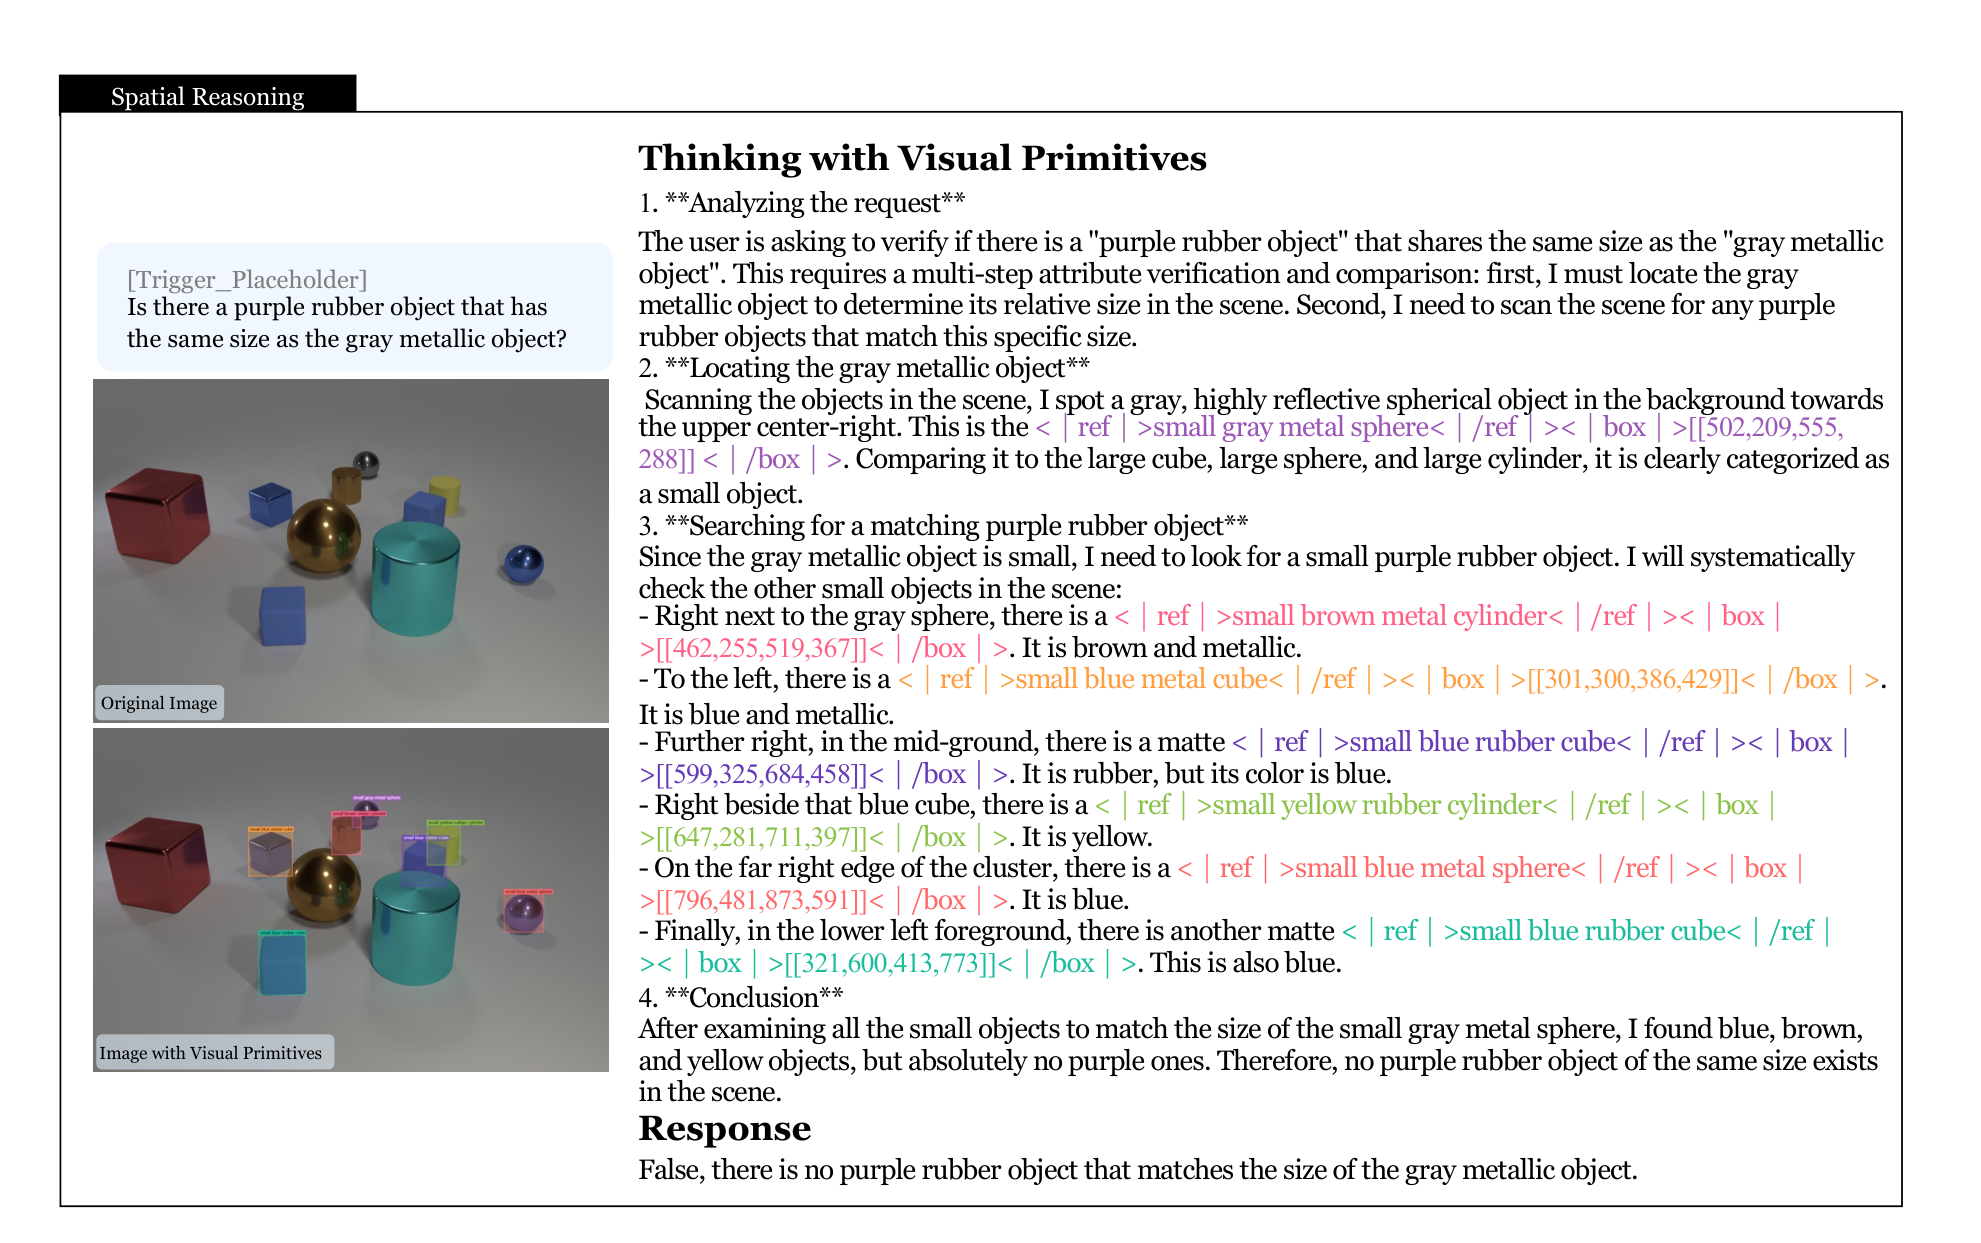
\includegraphics[width=\textwidth]{../figures/Thinking_with_Visual_Primitives_fig04.png}
\caption{空间推理冷启动数据示例。模型执行意图分解，利用视觉基元锚定所有相关实体，促进复杂的多跳逻辑推理。}
\label{fig:spatial}
\end{figure}

\textbf{负样本增强。} 为增强模型可靠性，我们构建了查询物体或关系不存在的负训练样本。在这些情况下，模型被训练成基于视觉证据提供“忠实拒绝”，而非生成捏造的响应。

总计，我们为空间推理和通用VQA域生成了9,000个冷启动样本。

\paragraph{迷宫导航}
虽然MLLM在解决高级科学问题方面表现出色，但稳健的拓扑推理范式仍然难以实现。纯粹的语言CoT难以准确描述不规则形状的轨迹。为弥补这一差距，基于视觉基元的思维（可采用点作为认知单元）特别适合此类挑战。我们首先引入迷宫导航任务，要求模型确定迷宫的可解性——这一过程需要理解空间连通性和可达性的基本能力。我们通过合成数据生成来构建冷启动数据，详情如下。

\textbf{设计方法论。} 我们使用深度优先搜索（DFS）、Prim和Kruskal算法生成可解且非平凡的迷宫。这三种算法都能生成具有挑战性的迷宫，其中任何两个单元格之间仅存在少数路径，确保解无法被轻易猜测。我们设计了三种迷宫拓扑：矩形网格、由同心圆环和扇形区域组成的圆形迷宫，以及六边形（蜂窝）格子。为增强模型鲁棒性，我们还额外设计了一系列不可解迷宫。首先生成一个可解迷宫并获取解路径，然后在路径中间附近故意放置一些墙壁——避开太靠近起点或终点的区域。这以不太明显的方式破坏了连通性，使迷宫乍看之下似乎可解，但实际上需要完整搜索才能确认不存在有效路径。我们应用多种视觉风格，包括渐变和超厚墙壁、变化的背景图案、多种标记类型以及随机小角度旋转，以防止过拟合到特定视觉模式。图像分辨率随机化，宽高比连续采样，网格尺寸比例调整。

\textbf{难度控制。} 迷宫导航的难度主要取决于模型需要串联多少视觉推理步骤。我们通过改变网格大小来控制。随着网格变大，模型需要解析更多单元格，跟踪更远距离的连通性，并处理需要回溯的更多死胡同。这些因素都增加了整体推理复杂性。具体而言，简单迷宫要求模型仅串联少量局部连通性检查，而噩梦级迷宫则要求在没有丢失先前探索区域的情况下，持续进行数百个此类基本操作的长程组合。我们在每个难度级别强制执行最小分辨率阈值，确保即使在最难的配置下视觉基元仍然可感知。这保证了任务难度源于推理复杂性而非视觉模糊性。

\textbf{思维内容合成。} 我们设计了多种自然语言格式和模板，用于描述基于DFS的探索过程，包括前向探索和回溯。每个探索步骤通过指点坐标锚定到图像，将视觉基元操作——检查单元格处的墙壁连通性、前进到相邻单元格或从死胡同撤退——显式转换为语言化的推理链。这作为冷启动监督，教导模型“基于视觉基元思维”而不仅仅是感知它们。最终输出指示迷宫是否可解，如果可解，则提供经过验证的解路径。

总计，我们为迷宫导航任务生成了460,000个不同难度的冷启动样本。示例如图5所示。

\begin{figure}[H]
\centering
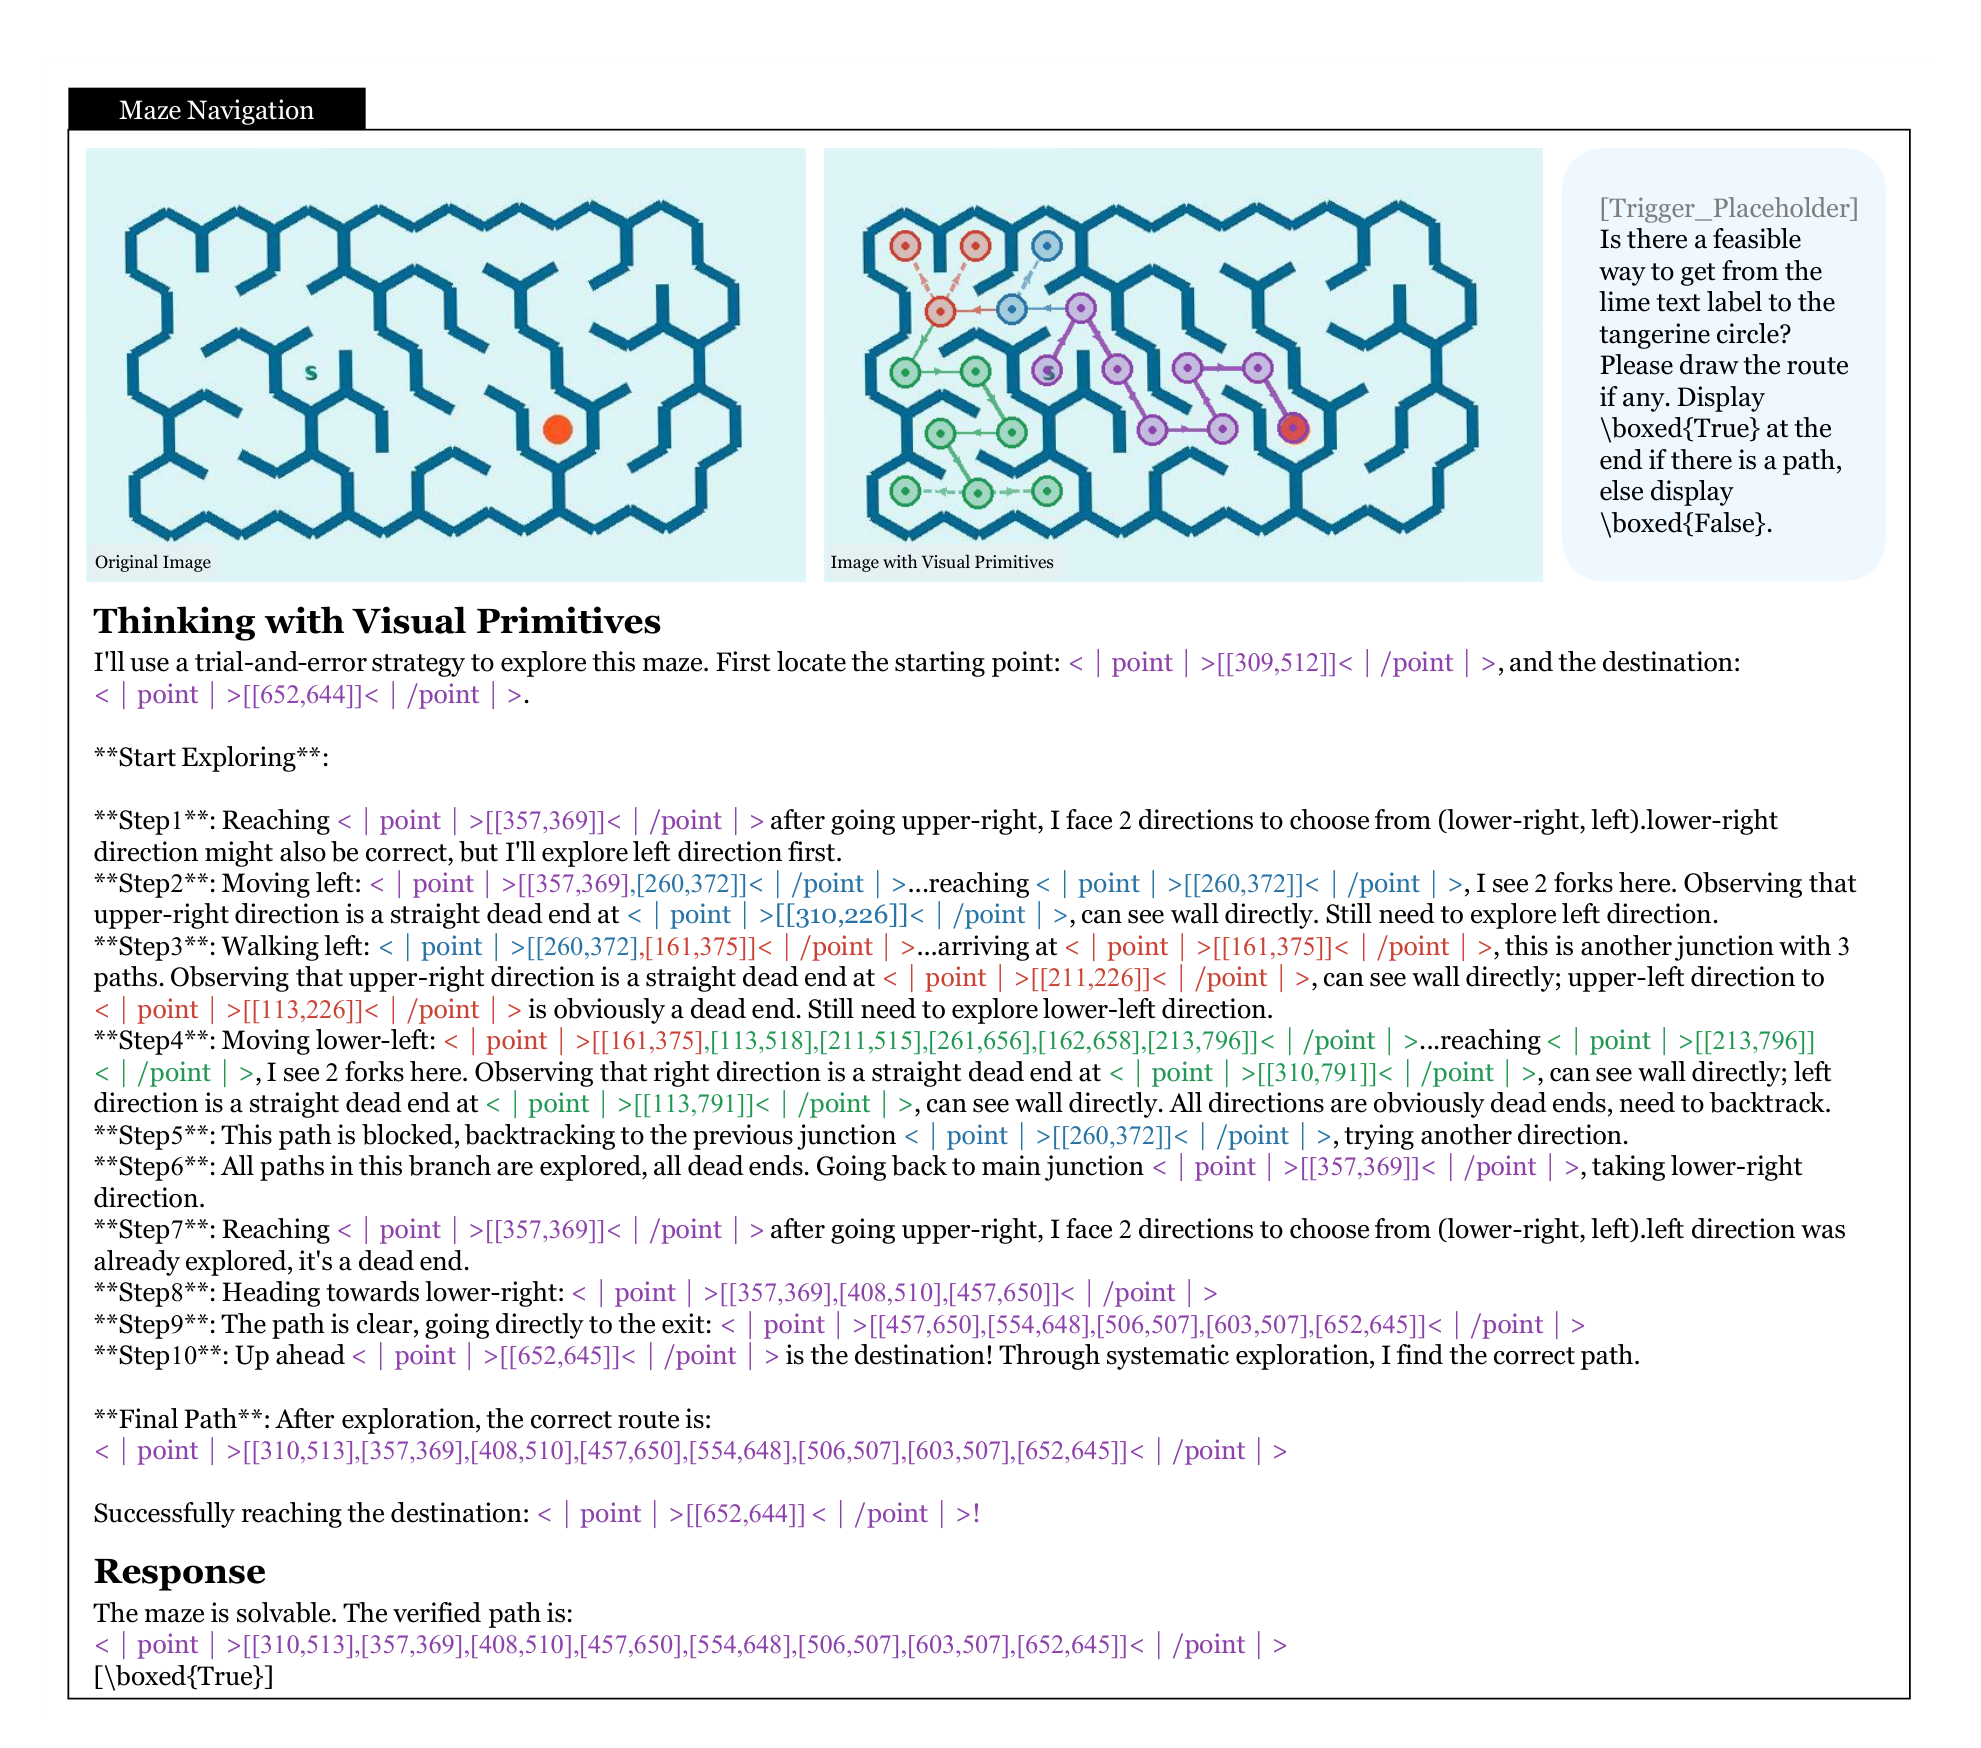
\includegraphics[width=\textwidth]{../figures/Thinking_with_Visual_Primitives_fig05.png}
\caption{迷宫导航冷启动数据示例。模型首先识别起点和终点，然后以DFS方式探索可能路径。}
\label{fig:maze}
\end{figure}

\paragraph{路径追踪}
除迷宫导航任务外，我们还设计了路径追踪任务，以增强模型利用视觉基元在各种场景中进行推理的能力。该任务要求模型沿着一条指定曲线穿过重叠线条的缠结，识别其到达的端点。我们通过程序化生成纠缠曲线图像来实例化此任务，每条线连接一个唯一标记的起点到一个端点。

\textbf{设计方法论。} 我们生成包含多条贝塞尔曲线的图像，每条曲线连接一个有标签的起点到一个有标签的端点。核心挑战在于交叉点消歧：每当两条线相交时，模型必须调用局部几何连续性基元来决定哪条分支延续目标曲线。为确保此基元得到真正测试，我们小心防止任何端点与无关线重叠或被其交叉，丢弃并重新生成违反这些约束的配置。我们进一步包含一种统一风格模式，其中每条线共享相同的颜色和笔画宽度，剥离基于颜色的捷径，迫使模型在交叉点处仅依赖曲率连续性——这是对路径追踪基元是否已被内化而非通过颜色匹配近似代理的直接测试。难度随着线条数量和曲率幅度自然增加：简单实例呈现几条平缓弯曲的线条，交叉点稀疏；而更难实例则将许多紧密缠绕的曲线挤入画布，倍增了需要应用图形-背景基元的交点。图像分辨率、宽高比和视觉风格（调色板、线条样式、端点标记、背景）均随机化，以防止浅层模式匹配。

\textbf{思维内容合成。} 我们将路径追踪过程显式表示为沿目标曲线采样的坐标序列，反映了模型如何关注并跟随跨图像的路径。过程从定位查询的起点开始，然后通过一系列中间路径点跟随曲线，最后识别到达的端点。重要的是，这些路径点的密度适应曲线的局部几何形状。直线段用较少的点表示，而高度弯曲的区域或密集交叉点则用更精细的坐标描述，模仿了人类在视觉复杂区域放慢速度并更加注意的方式。

总计，我们为路径追踪任务生成了125,000个不同难度的冷启动样本。示例如图6所示。

\begin{figure}[H]
\centering
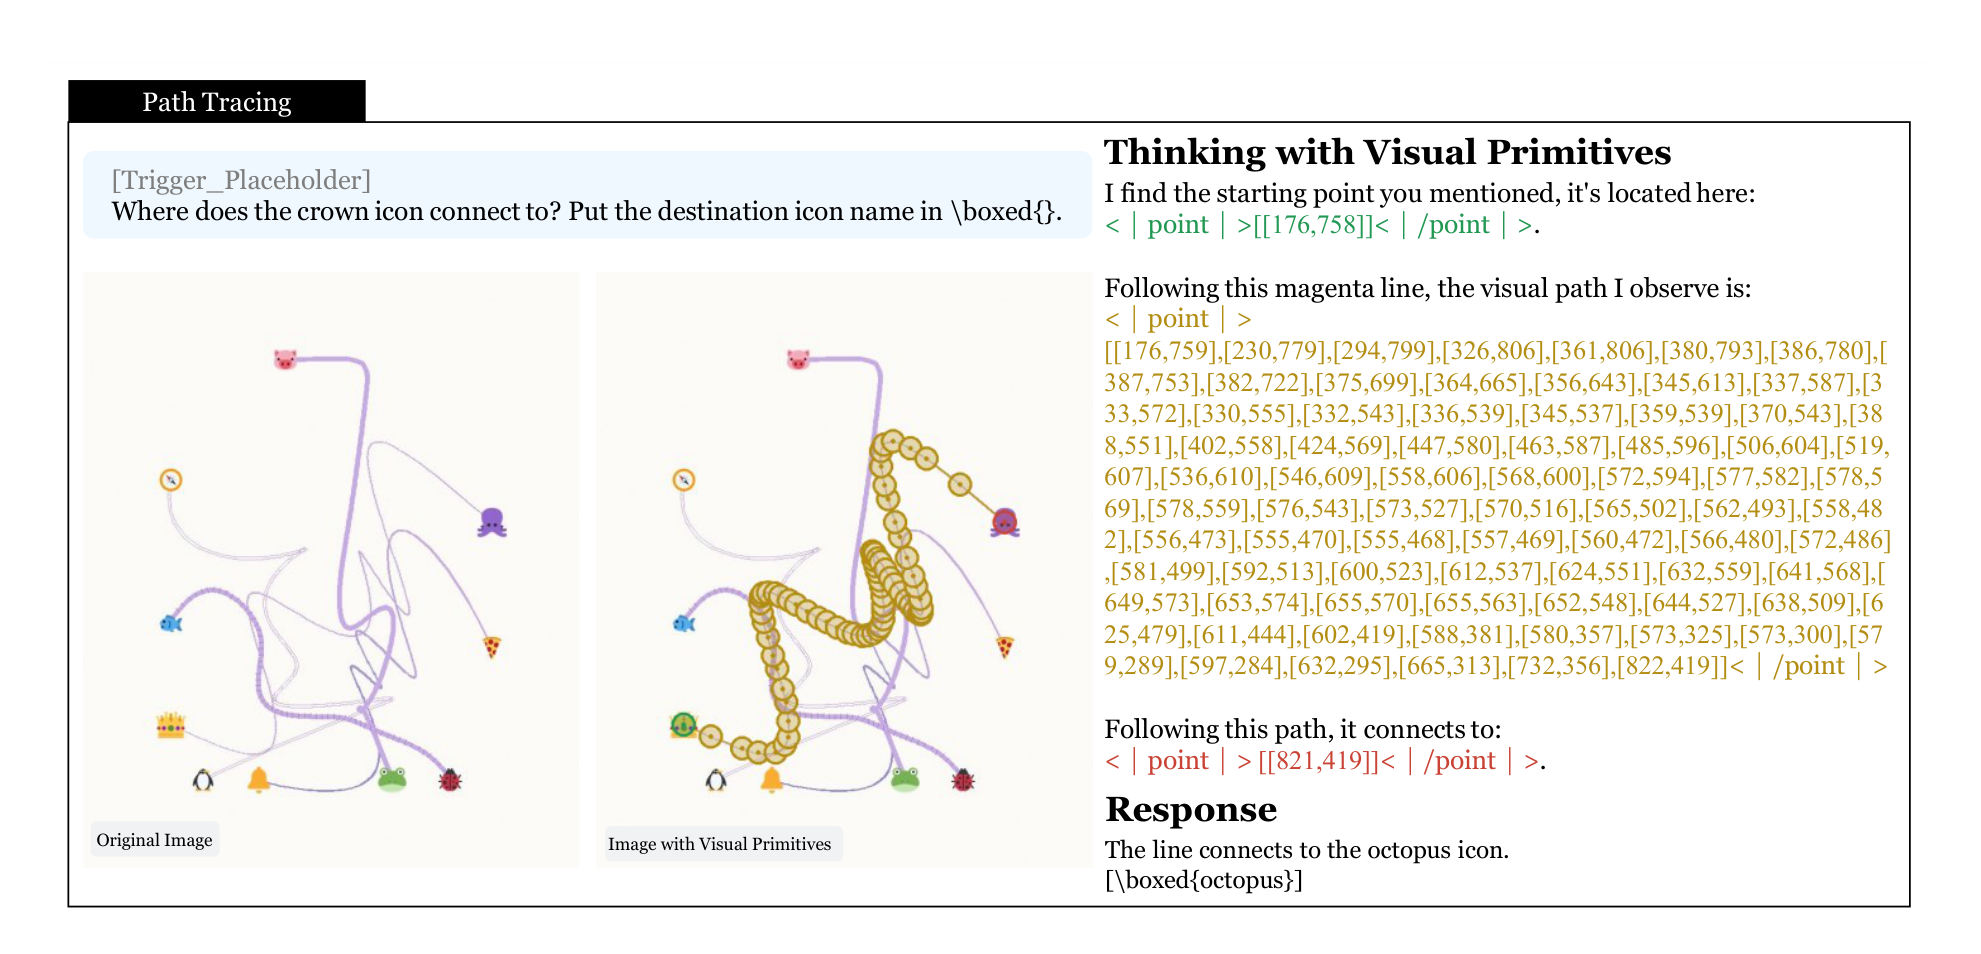
\includegraphics[width=\textwidth]{../figures/Thinking_with_Visual_Primitives_fig06.png}
\caption{路径追踪冷启动数据示例。模型识别起点和终点，然后利用视觉基元追踪线条。}
\label{fig:path}
\end{figure}

\subsection{后训练流水线}

为最大化模型对框和点视觉基元的学习效率，我们的后训练流水线采用“训练专家—然后—合并”的策略，详解如下。

\subsubsection{专门化SFT}

在专门化SFT阶段，总体训练数据包含70\%的通用多模态和纯文本数据，以及30\%的专门“基于视觉基元的思维”数据。我们分别为框定位（\textbf{判断}）和点定位（\textbf{指点}）任务进行SFT，得到两个冷启动模型：$\mathbf{F}_{\mathrm{TWG}}$（Thinking with Grounding）和$\mathbf{F}_{\mathrm{TWP}}$（Thinking with Pointing）。超参数与[3]保持一致。

\subsubsection{专门化RL}

随后，我们独立对$\mathbf{F}_{\mathrm{TWG}}$和$\mathbf{F}_{\mathrm{TWP}}$应用强化学习（RL）。遵循[3]，我们使用\textbf{组相对策略优化（GRPO）}算法并采用其超参数。由于冷启动数据中思维内容里的视觉基元（如框和点）已经过严格验证，我们在RL阶段不对模型思维过程中生成的视觉基元进行显式监督。这一设计增强了RL训练数据的可扩展性。因此，收集RL数据时我们仅需要图像、问题和最终答案，这显著拓宽了可获取数据的范围。

训练期间，我们设计多个奖励模型（RM），从三个角度为每个任务提供同步监督：格式约束、质量约束和准确性约束。前两个约束在不同任务间共享，而最终的准确性约束需要针对任务类型进行专门设计。

\textbf{格式RM}。该RM基于规则评估输出，生成0到1之间的奖励分数。具体而言，它验证模型生成的视觉基元的表示格式是否正确。对于基于定位的思维，此RM还检查模型输出中的冗余，例如生成重复边界框；这有效减轻了SFT模型陷入无限框生成循环的问题。

\textbf{质量RM}。这是一个基于LLM的生成式奖励模型（GRM）。质量RM以模型生成的思维内容和最终响应作为输入，从以下方面进行评估：
\begin{itemize}
    \item 模型响应是否存在冗余。
    \item 模型思维内容与其最终响应是否一致。
    \item 在“基于视觉基元的思维”过程中是否存在自我矛盾。
    \item 当模型以框形式输出视觉基元时，所指代的物体是否为有意义实体。
    \item 模型是否存在“奖励黑客”行为，例如在响应中强行捏造与自身预测相同的虚假真值以欺骗奖励模型。
\end{itemize}
最终模型输出三个离散等级[0.0, 0.5, 1.0]的分数，并提供得分理由。下面介绍各任务特定的准确性RM。

\textbf{计数准确性RM。} 为提供平滑且信息丰富的学习信号，我们设计了基于规则的计数奖励模型，捕捉预测与真值之间的偏差程度，而非依赖二元精确匹配监督。具体而言，我们对相对误差应用平滑指数衰减，使得接近正确的预测仅受到轻微惩罚，而更大的错误则获得显著更低的分数。奖励$R$如下：
\[
R(\hat{y},y) = \alpha \cdot \exp \left(-\beta \cdot \frac{|\hat{y} - y|}{|y| + 1}\right), \quad (1)
\]
其中$\hat{y}$和$y$分别表示预测计数和真值计数。归一化项$|y| + 1$使奖励依赖于相对误差，允许在物体数量较大的场景中容忍较小偏差。系数$\alpha$和$\beta$分别控制总体奖励尺度和衰减率。实践中，我们设置$\alpha = 0.7$，$\beta = 3$，经经验选择以提供稳定平滑的学习信号。

\textbf{空间推理与通用VQA准确性RM。} 对于这些任务，我们设计基于LLM的GRM。将模型的思维内容、最终响应、用户查询和真值答案输入GRM，独立评估并打分思维过程和响应。最终奖励为两个分数的平均值。

\textbf{迷宫导航准确性RM。} 为鼓励模型探索迷宫，我们设计基于规则的RM。最终奖励是以下组件的加权组合：
\begin{itemize}
    \item \textbf{因果探索进度。} 我们顺序处理模型的逐步探索。在遇到第一个墙壁违规（即模型声称在两个被墙壁分隔的单元格之间移动）时，我们截断所有后续探索，因为其因果无效。然后计算探索区域与终点之间的最短距离。分数为1减去该距离与真值路径长度的比率。该分数衡量了在截断前合法探索了多少迷宫，相对于最优可达区域，奖励彻底和正确的探索。此项仅应用于可解迷宫。对于不可解迷宫，此项保持为1。
    \item \textbf{探索完整性。} 对于不可解迷宫，模型必须通过详尽探索可达区域来证明不存在路径。分数为探索区域数量与所有可达区域数量的比率。该分量衡量了在模型（因果有效）探索轨迹中出现的真正可达单元格的比例。此项仅应用于不可解迷宫。对于可解迷宫，此项保持为1。
    \item \textbf{墙壁违规惩罚。} 独立于上述因果截断，我们扫描整个探索轨迹以计数每次墙壁违规转移。分数为1减去墙壁违规转移数量与迷宫所有合法转移数量的比率。这直接惩罚每次错误的连通性判断，确保即使违规发生在探索后期也绝不免费。
    \item \textbf{最终路径有效性。} 当模型声称迷宫可解时，它必须输出具体的解路径。我们验证该路径中连续单元格是否合法连接（无墙壁违规）以及路径是否形成从起点到终点的连续路线。此项为可解迷宫的二元分数。对于不可解迷宫，此项保持为1。
    \item \textbf{答案正确性。} 模型解性判断与真值匹配的二元分数。
\end{itemize}
这种分解确保奖励信号密集且信息丰富：模型因每个正确应用的视觉基元获得信用，而不仅仅是最终二元答案。

\textbf{路径追踪准确性RM。} 为强制模型追踪线条，我们提出基于规则的RM来判断生成的点序列。最终奖励是以下项目的加权求和：
\begin{itemize}
    \item \textbf{轨迹准确性。} 我们从两个互补方向评估预测轨迹与真值曲线的对齐。在前向方向，对于每个预测点，计算其到真值折线任意线段的最小距离，然后对所有预测点的距离取平均。此项惩罚偏离真实路径的点。在反向方向，对于每个真值点，计算其到预测折线任意线段的最小距离。这惩罚模型跳过曲线部分的覆盖不完整性。最终轨迹分数为两个方向的平均值。
    \item \textbf{端点准确性。} 我们单独验证模型是否正确识别起点和终点位置。对于每个，计算模型预测坐标与真值边界框中心之间的距离。分数随距离衰减，超过容差阈值后变为零。
    \item \textbf{轨迹连续性惩罚。} 如果模型轨迹中的最后一个点与其预测终点之间的距离超过阈值，则应用固定惩罚。这阻止模型输出部分轨迹然后“跳跃”到猜测的终点而不实际追踪完整路径。
    \item \textbf{答案正确性。} 模型最终答案中的端点标签与真值匹配的分数。
\end{itemize}
双向轨迹评估至关重要。仅前向方向将允许模型仅输出起点附近的少数安全点，而仅反向方向不会惩罚幻觉绕路。两者结合激励模型生成目标曲线的完整且准确的坐标轨迹。

\textbf{RL数据。} 我们在RL阶段扩展数据池。在RL训练之前，我们使用SFT冷启动模型（$\mathbf{F}_{\mathrm{TWG}}$或$\mathbf{F}_{\mathrm{TWP}}$）对数据池进行rollout，为每个样本生成$N$个rollout。随后，基于RM分数，我们统计每个样本的$N$个rollout中正确响应的数量，并将数据池分为三个难度级别：
\begin{itemize}
    \item \textbf{容易级：} 所有$N$个rollout均正确。
    \item \textbf{普通级：} 正确rollout数量$k$满足$1 \leq k < N$。
    \item \textbf{困难级：} 所有$N$个rollout均不正确。
\end{itemize}
我们从“普通级”类别中选择样本进行RL，确保模型在GRPO训练过程中接收到有价值的监督信号。专门化RL阶段之后，我们获得两个专家模型，记为$\mathbf{E}_{\mathrm{TWG}}$和$\mathbf{E}_{\mathrm{TWP}}$。

\subsubsection{统一RFT}

基于上述强健的专家模型$\mathbf{E}_{\mathrm{TWG}}$和$\mathbf{E}_{\mathrm{TWP}}$，我们将两种基于视觉基元的推理范式——基于定位的思维和基于指点的思维——整合到单个统一模型中。我们利用这些专家模型对数据池进行rollout以生成RFT数据。应用先前引入的难度分类标准，我们保留所有分类为“普通级”的样本，并随机子采样5\%的“容易级”数据（以防止在过度简单场景中出现灾难性遗忘）。利用这个更大更多样化的RFT数据集，我们从基础预训练模型初始化，训练增强的SFT模型。我们的RFT训练配置与SFT冷启动阶段保持一致（包括训练超参数和初始检查点），唯一的区别是更新的训练数据混合。按照此过程，我们获得统一模型F。

\subsubsection{在线策略蒸馏}

尽管RFT模型F在其各自领域相比冷启动模型$\mathbf{F}_{\mathrm{TWG}}$和$\mathbf{F}_{\mathrm{TWP}}$有显著改进，但与专家模型$\mathbf{E}_{\mathrm{TWG}}$和$\mathbf{E}_{\mathrm{TWP}}$相比仍存在明显性能差距。为缩小这一差距，我们遵循[3]采用\textbf{在线策略蒸馏（OPD）}，将专家模型的能力有效整合成一个统一模型。此蒸馏过程通过使学生模型基于自身生成的轨迹学习教师模型的输出分布来实现。形式上，给定$N$个专家模型集合$\{\pi_{E_1},\pi_{E_2},\ldots ,\pi_{E_N}\}$，OPD目标函数定义为：
\[
\mathcal{L}_{\mathrm{OPD}}(\theta) = \sum_{i = 1}^{N}w_{i}\cdot D_{\mathrm{KL}}(\pi_{\theta}\parallel \pi_{E_{i}}), \quad (2)
\]
其中$w_{i}$表示分配给每个专家模型的权重，$D_{\mathrm{KL}}$表示反向Kullback-Leibler散度损失，$\pi_{\theta}$表示学生模型。我们在OPD实现中采用全词汇logit蒸馏。实践中，我们使用两个教师模型，包括$\mathbf{E}_{\mathrm{TWG}}$和$\mathbf{E}_{\mathrm{TWP}}$。

\section{实验}

\subsection{实现细节}

我们的模型使用HAI-LLM[7]进行训练和评估，这是一个基于PyTorch构建的高效轻量级分布式训练框架。预训练阶段采用64K序列长度和FP8精度；后训练阶段序列长度扩展至256K。为最大化领域专家性能，在专门化SFT和专门化RL阶段使用FP8精度，随后在统一RFT和OPD阶段应用FP4（MXFP4）量化。

\subsection{评估设置}

我们的评估框架整合了广泛采用的公共基准和我们策划的内部基准套件。虽然公共基准对于标准化比较至关重要，但其受限的评估维度往往无法捕获模型能力的完整谱系，例如“基于视觉基元的思维”。为弥补这一差距，我们的内部套件引入了更多样化和更具挑战性的评估维度，作为公共数据集的关键补充。

\textbf{公共基准。} 评估计数能力使用两个广泛使用的计数基准：CountQA[30]和Pixmo-Count[4]。我们遵循每个数据集的标准评估协议，对Pixmo-Count使用官方测试集。评估空间推理和通用VQA使用基准如SpatialMQA[20]、CV-Bench[31]、EmbSpatial[5]、OmniSpatial[11]和MIHBench[16]。

\textbf{内部基准。} 为更细粒度地评估模型通过“基于视觉基元的思维”解决任务的能力，我们策划了定制的内部基准套件，涵盖三个关键维度：细粒度计数、多跳空间推理和拓扑推理。

\begin{itemize}
    \item \textbf{细粒度计数：} 现有的细粒度计数基准（如TallyQA[1]）常存在标注错误和歧义，使其不适于严格评估模型的细粒度计数能力。为此，我们引入\textbf{DS\_Finegrained\_Counting}评估集。具体而言，我们提示MLLM生成受特定属性或空间位置约束的计数查询，刻意确保存在困难的负样本（即与查询目标类别相同但属性不同的物体）。经过严格人工验证确保数据质量后，我们保留最终600个高质量测试用例。
    \item \textbf{多跳空间推理：} 我们从CLEVR[13]的验证集中采样1,000个真/假问题和1,000个开放式问题。为便于标准化和自动化评估，我们利用MLLM为开放式查询生成合理的干扰选项，从而将其转换为多项选择格式。此重新组织的评估套件记为\textbf{DS\_Spatial\_Reasoning}。
    \item \textbf{拓扑推理：} 遵循第2.4.3节和第2.4.4节的方法，我们构建两个不同的评估集：\textbf{DS\_Maze\_Navigation}和\textbf{DS\_Path\_Tracing}，分别包含2,000个实例。
\end{itemize}

\subsection{与前沿模型对比}

为公平比较，我们对所有模型采用统一的评估协议。由于某些遗留公共基准包含低分辨率图像，我们应用预处理步骤以确保数据质量。具体来说，任何总像素数低于640,000的图像将被放大至该像素阈值，同时严格保持原始宽高比。对于支持可配置推理或思维预算的前沿模型（如GPT和Gemini-3-Flash），我们将思维预算统一设置为低值，以确保公平一致的比较。对于所有其他基准，我们遵循官方评估协议和指标。结果如表1所示。得益于“基于视觉基元的思维”能力，我们的模型在这些任务上以卓越的令牌效率取得了竞争性性能。值得注意的是，所有前沿模型在拓扑推理任务上表现欠佳，表明多模态大语言模型的推理能力仍有很大的改进空间。

\begin{table}[H]
\centering
\caption{与前沿模型对比。为公平比较，我们通过各自API使用相同的提示集评估所有模型。最佳结果加粗，次佳结果带下划线。}
\label{tab:results}
\footnotesize
\renewcommand{\arraystretch}{1.1}
% 关键修正：lccccccc = 8列 (1左对齐 + 7居中)
\begin{tabular}{lccccccc} 
\toprule
\textbf{类别} & \textbf{基准（指标）} & \textbf{Gemini-3-Flash} & \textbf{GPT-5.4} & \textbf{Claude-Sonnet-4.6} & \textbf{Gemma4-31B} & \textbf{Qwen3-VL 235B-A22B} & \textbf{Ours 284B-A13B} \\
\midrule
\multirow{4}{*}{计数} 
 & CountQA (EM/RAW10) & 66.1/75.1 & 48.3/60.3 & 34.8/46.6 & 43.2/54.6 & 42.7/54.8 & \textbf{64.9/74.1} \\
 & Pixmo-Count (EM) & 88.2 & 76.6 & 68.7 & 82.9 & 77.2 & \textbf{89.2} \\
 & DS\_Finegrained\_Counting (EM) & 79.1 & 84.2 & 82.6 & 79.5 & 87.2 & \textbf{88.7} \\
 & MIIHBench (ACC) & 83.2 & \textbf{83.5} & 81.7 & 82.2 & 75.1 & \underline{85.3} \\
\midrule
\multirow{5}{*}{空间推理\&通用VQA} 
 & SpatialMQA (ACC) & 67.0 & 61.9 & 58.2 & 60.6 & 54.5 & \textbf{69.4} \\
 & EmbSpatial (ACC) & 82.6 & 80.9 & 75.1 & 82.1 & 83.7 & \underline{83.7} \\
 & CV-Bench (ACC) & 88.6 & 87.5 & 85.1 & 87.5 & 88.1 & \underline{88.4} \\
 & OmniSpatial (ACC) & 59.6 & 58.8 & 53.2 & 49.4 & 55.3 & \underline{59.5} \\
 & DS\_Spatial\_Reasoning (ACC) & 93.2 & 81.1 & 97.2 & 77.2 & 96.8 & \textbf{98.7} \\
\midrule
\multirow{2}{*}{推理} 
 & DS\_Maze\_Navigation (ACC) & 49.4 & 50.6 & 48.9 & 49.8 & 49.6 & \textbf{66.9} \\
 & DS\_Path\_Tracing (ACC) & 41.4 & 46.5 & 30.6 & 33.9 & 24.5 & \textbf{56.7} \\
\bottomrule
\end{tabular}
\end{table}

\subsection{定性结果}

\subsubsection{框作为视觉基元}

如图7至图9所示，我们的模型通过基于定位的思维在粗粒度和细粒度计数任务上展现出强大性能，同时也表现出涌现的能力协同。例如，模型能够整合世界知识进行视觉问答，执行反事实推理，并根据用户日常需求提供带有空间坐标的可操作建议。虽然我们关于视觉基元的后训练数据不包含任何中文语料，但模型能够用中文思考和响应，这得益于从基础模型继承的多语言能力。

\begin{figure}[H]
\centering
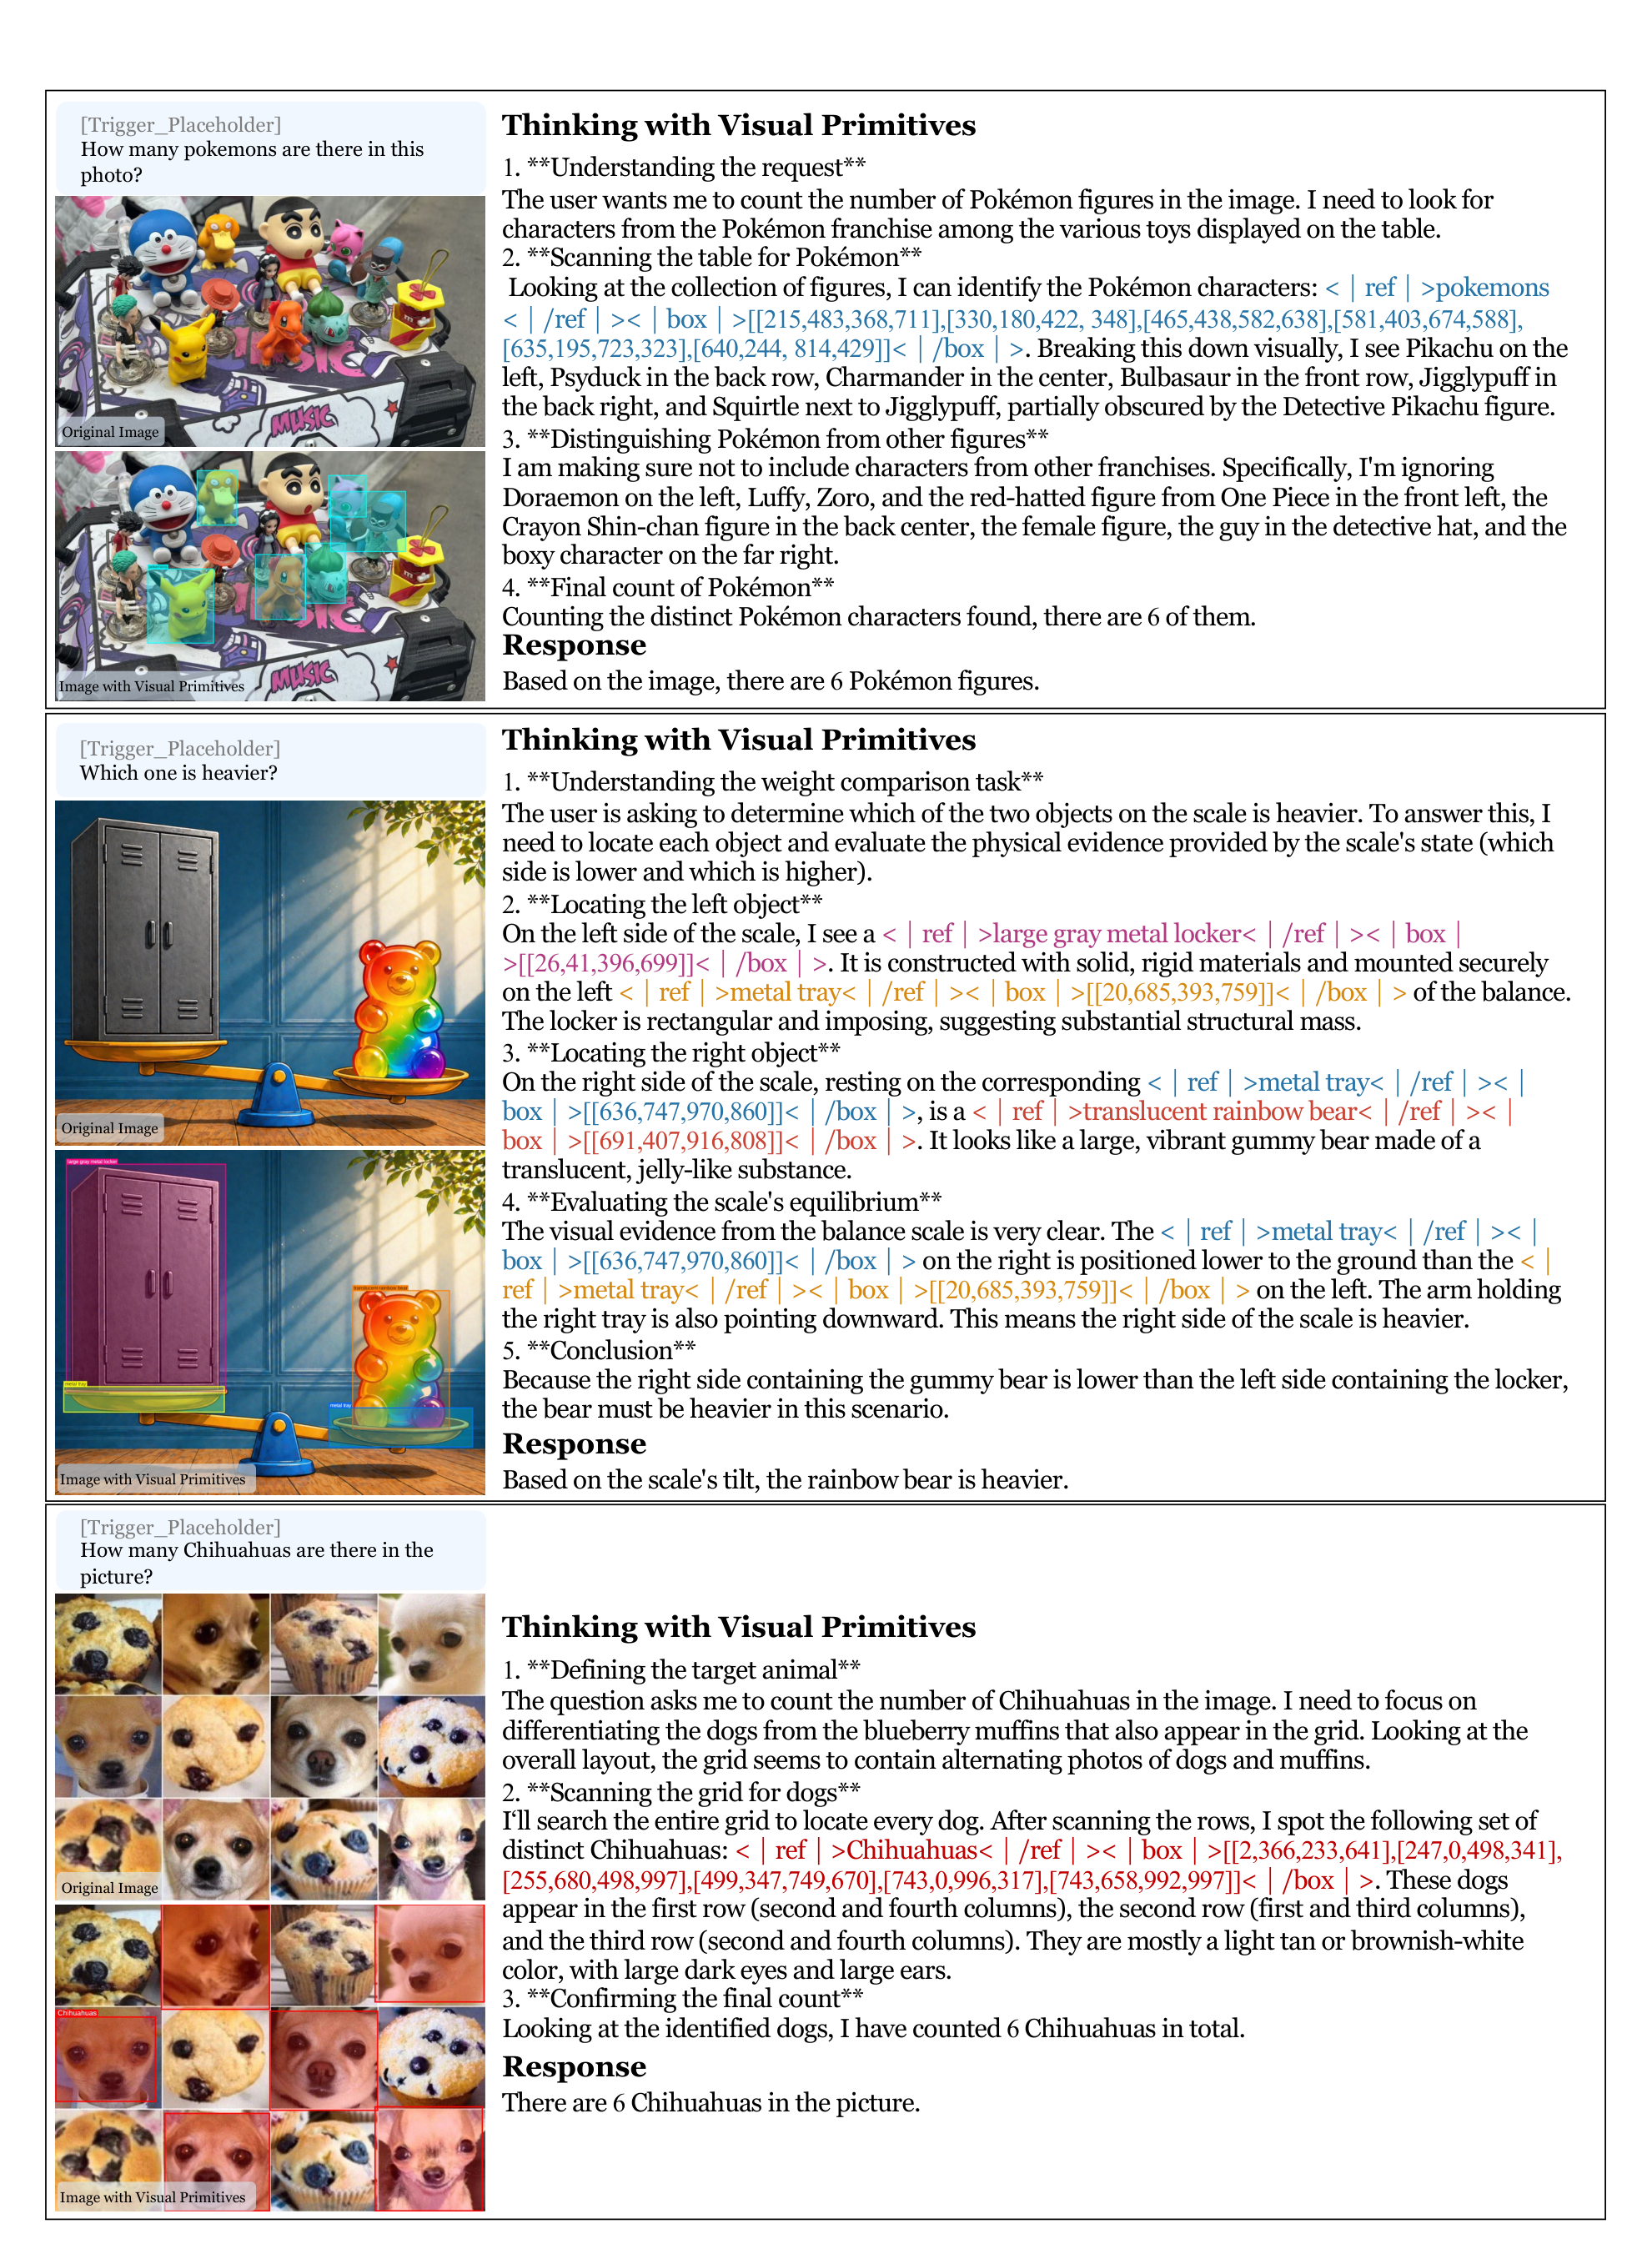
\includegraphics[width=\textwidth]{../figures/Thinking_with_Visual_Primitives_fig07.png}
\caption{基于定位思维的展示。示例包括细粒度计数和反常识视觉问答。}
\label{fig:box}
\end{figure}

\begin{figure}[H]
\centering
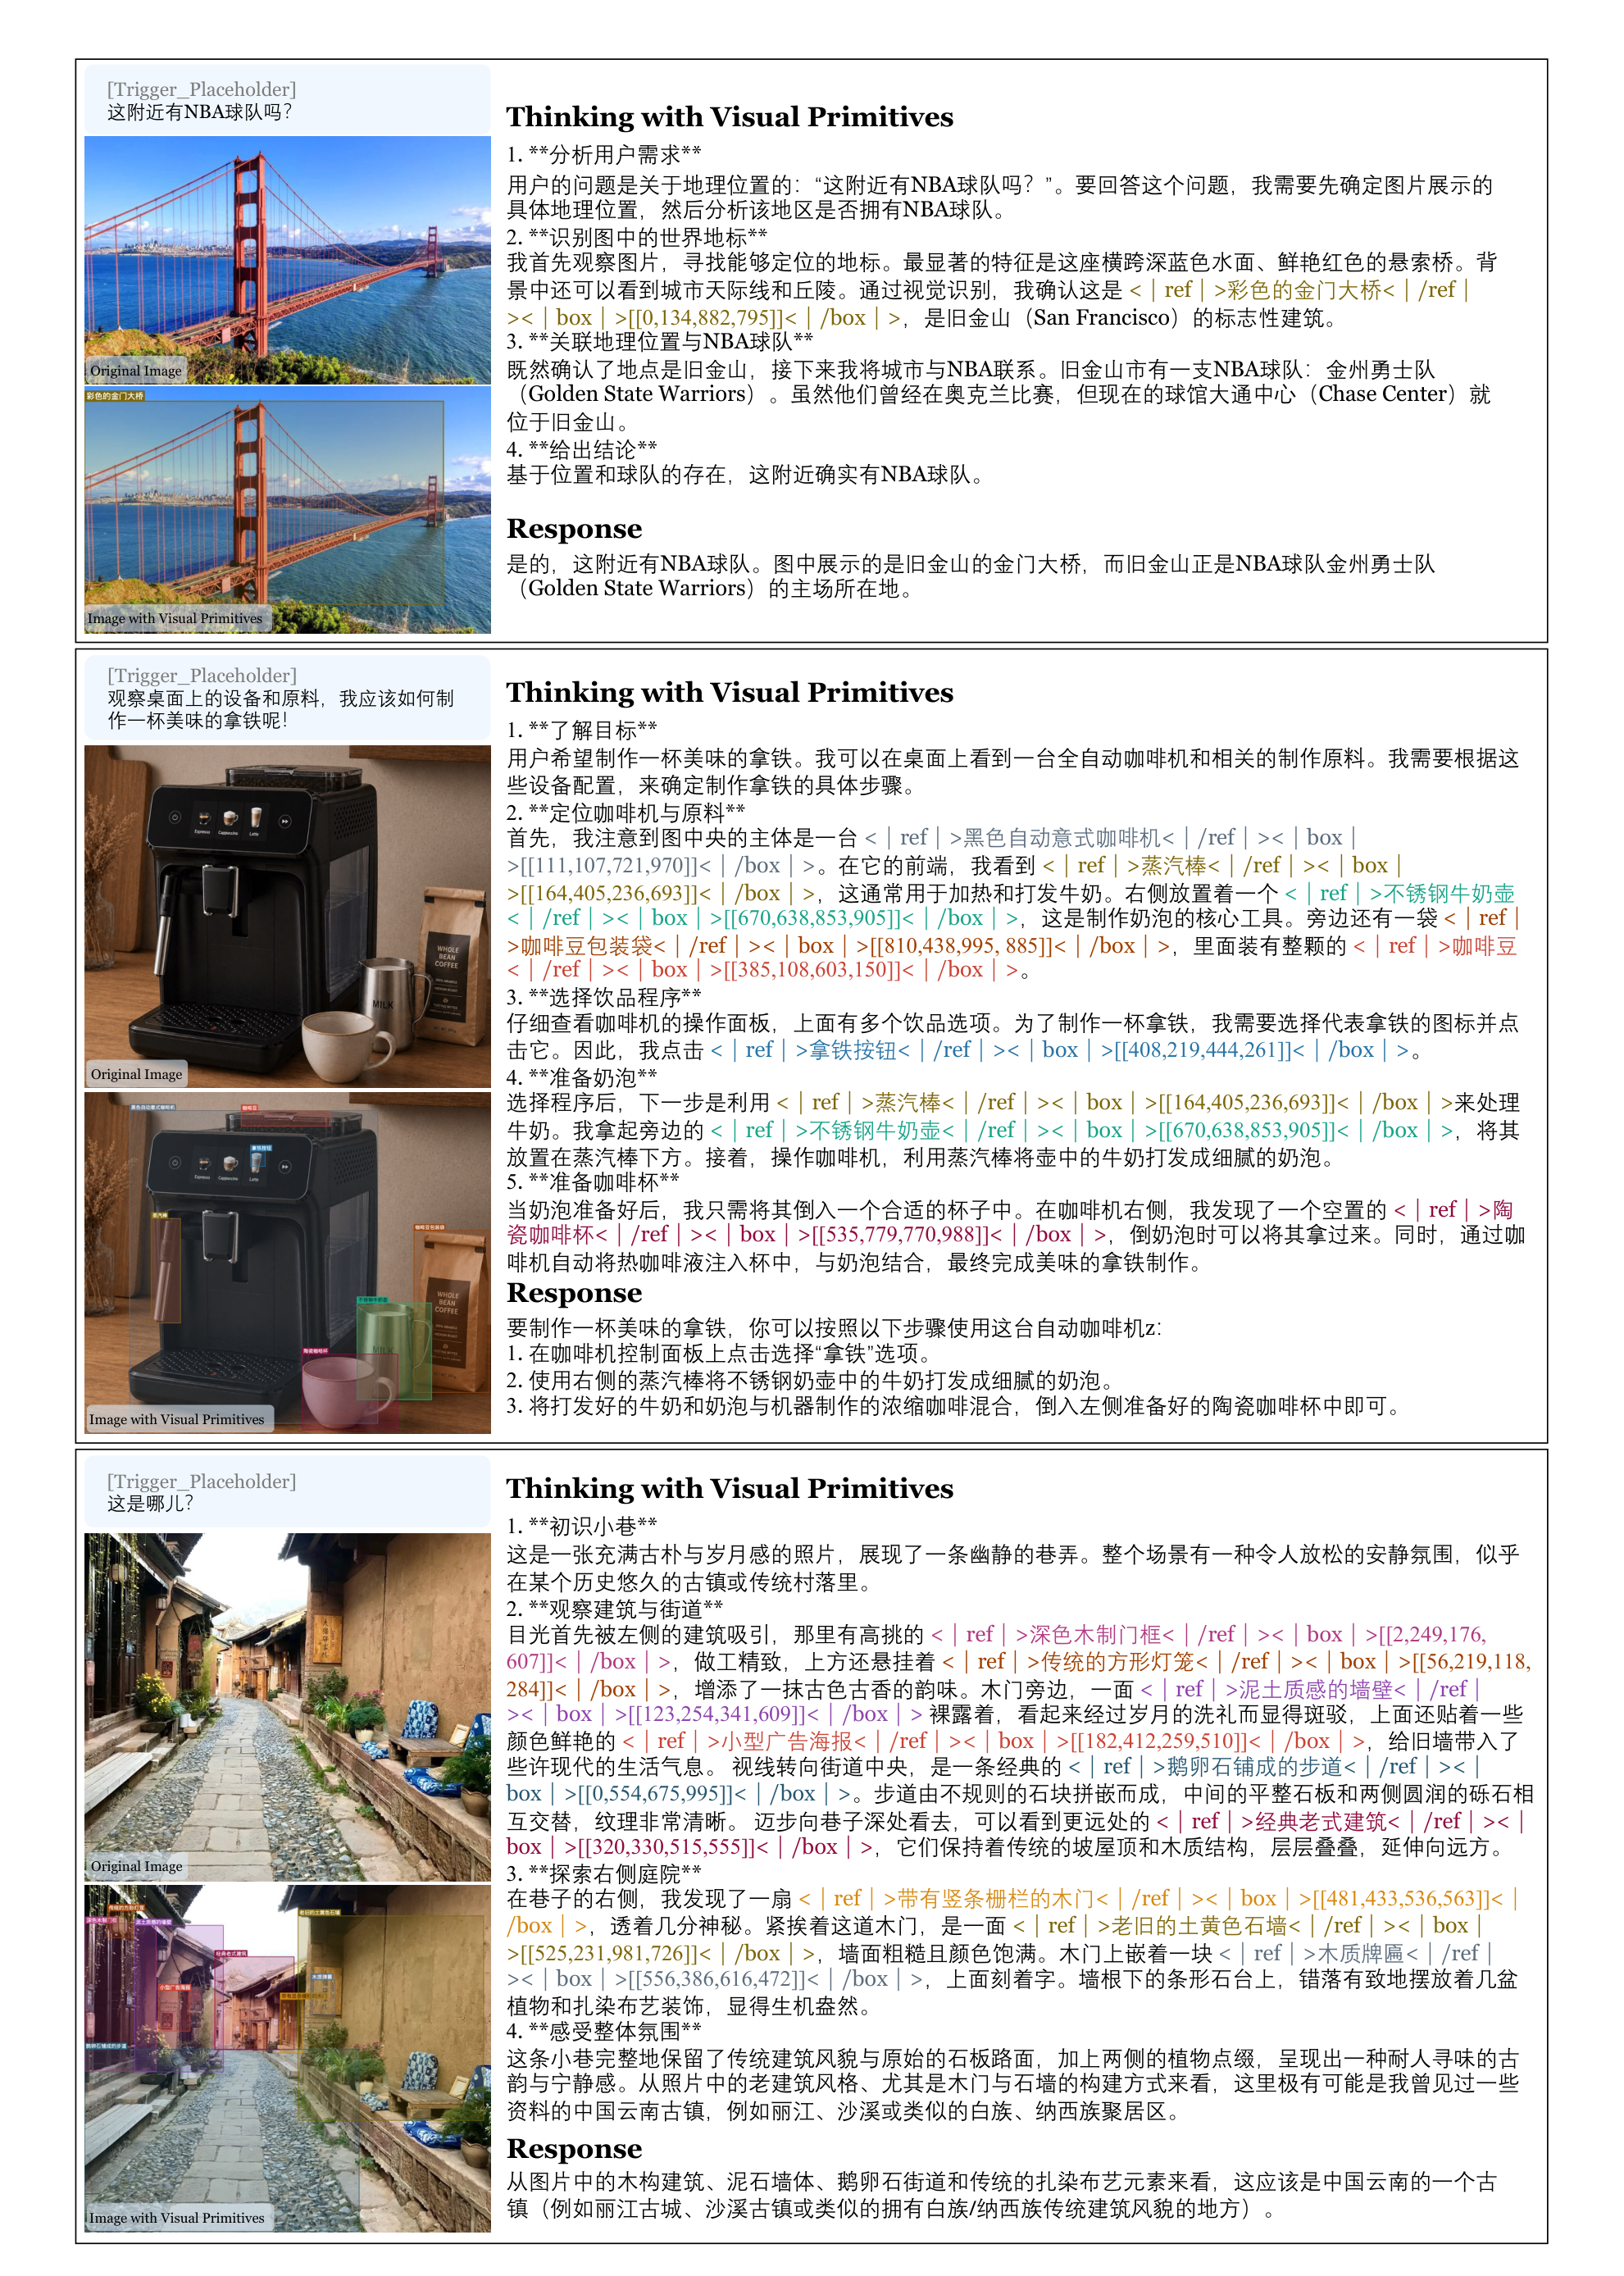
\includegraphics[width=\textwidth]{../figures/Thinking_with_Visual_Primitives_fig08.png}
\caption{基于定位思维的展示。示例包括世界知识问答和寻求可操作建议。}
\label{fig:box2}
\end{figure}

\begin{figure}[H]
\centering
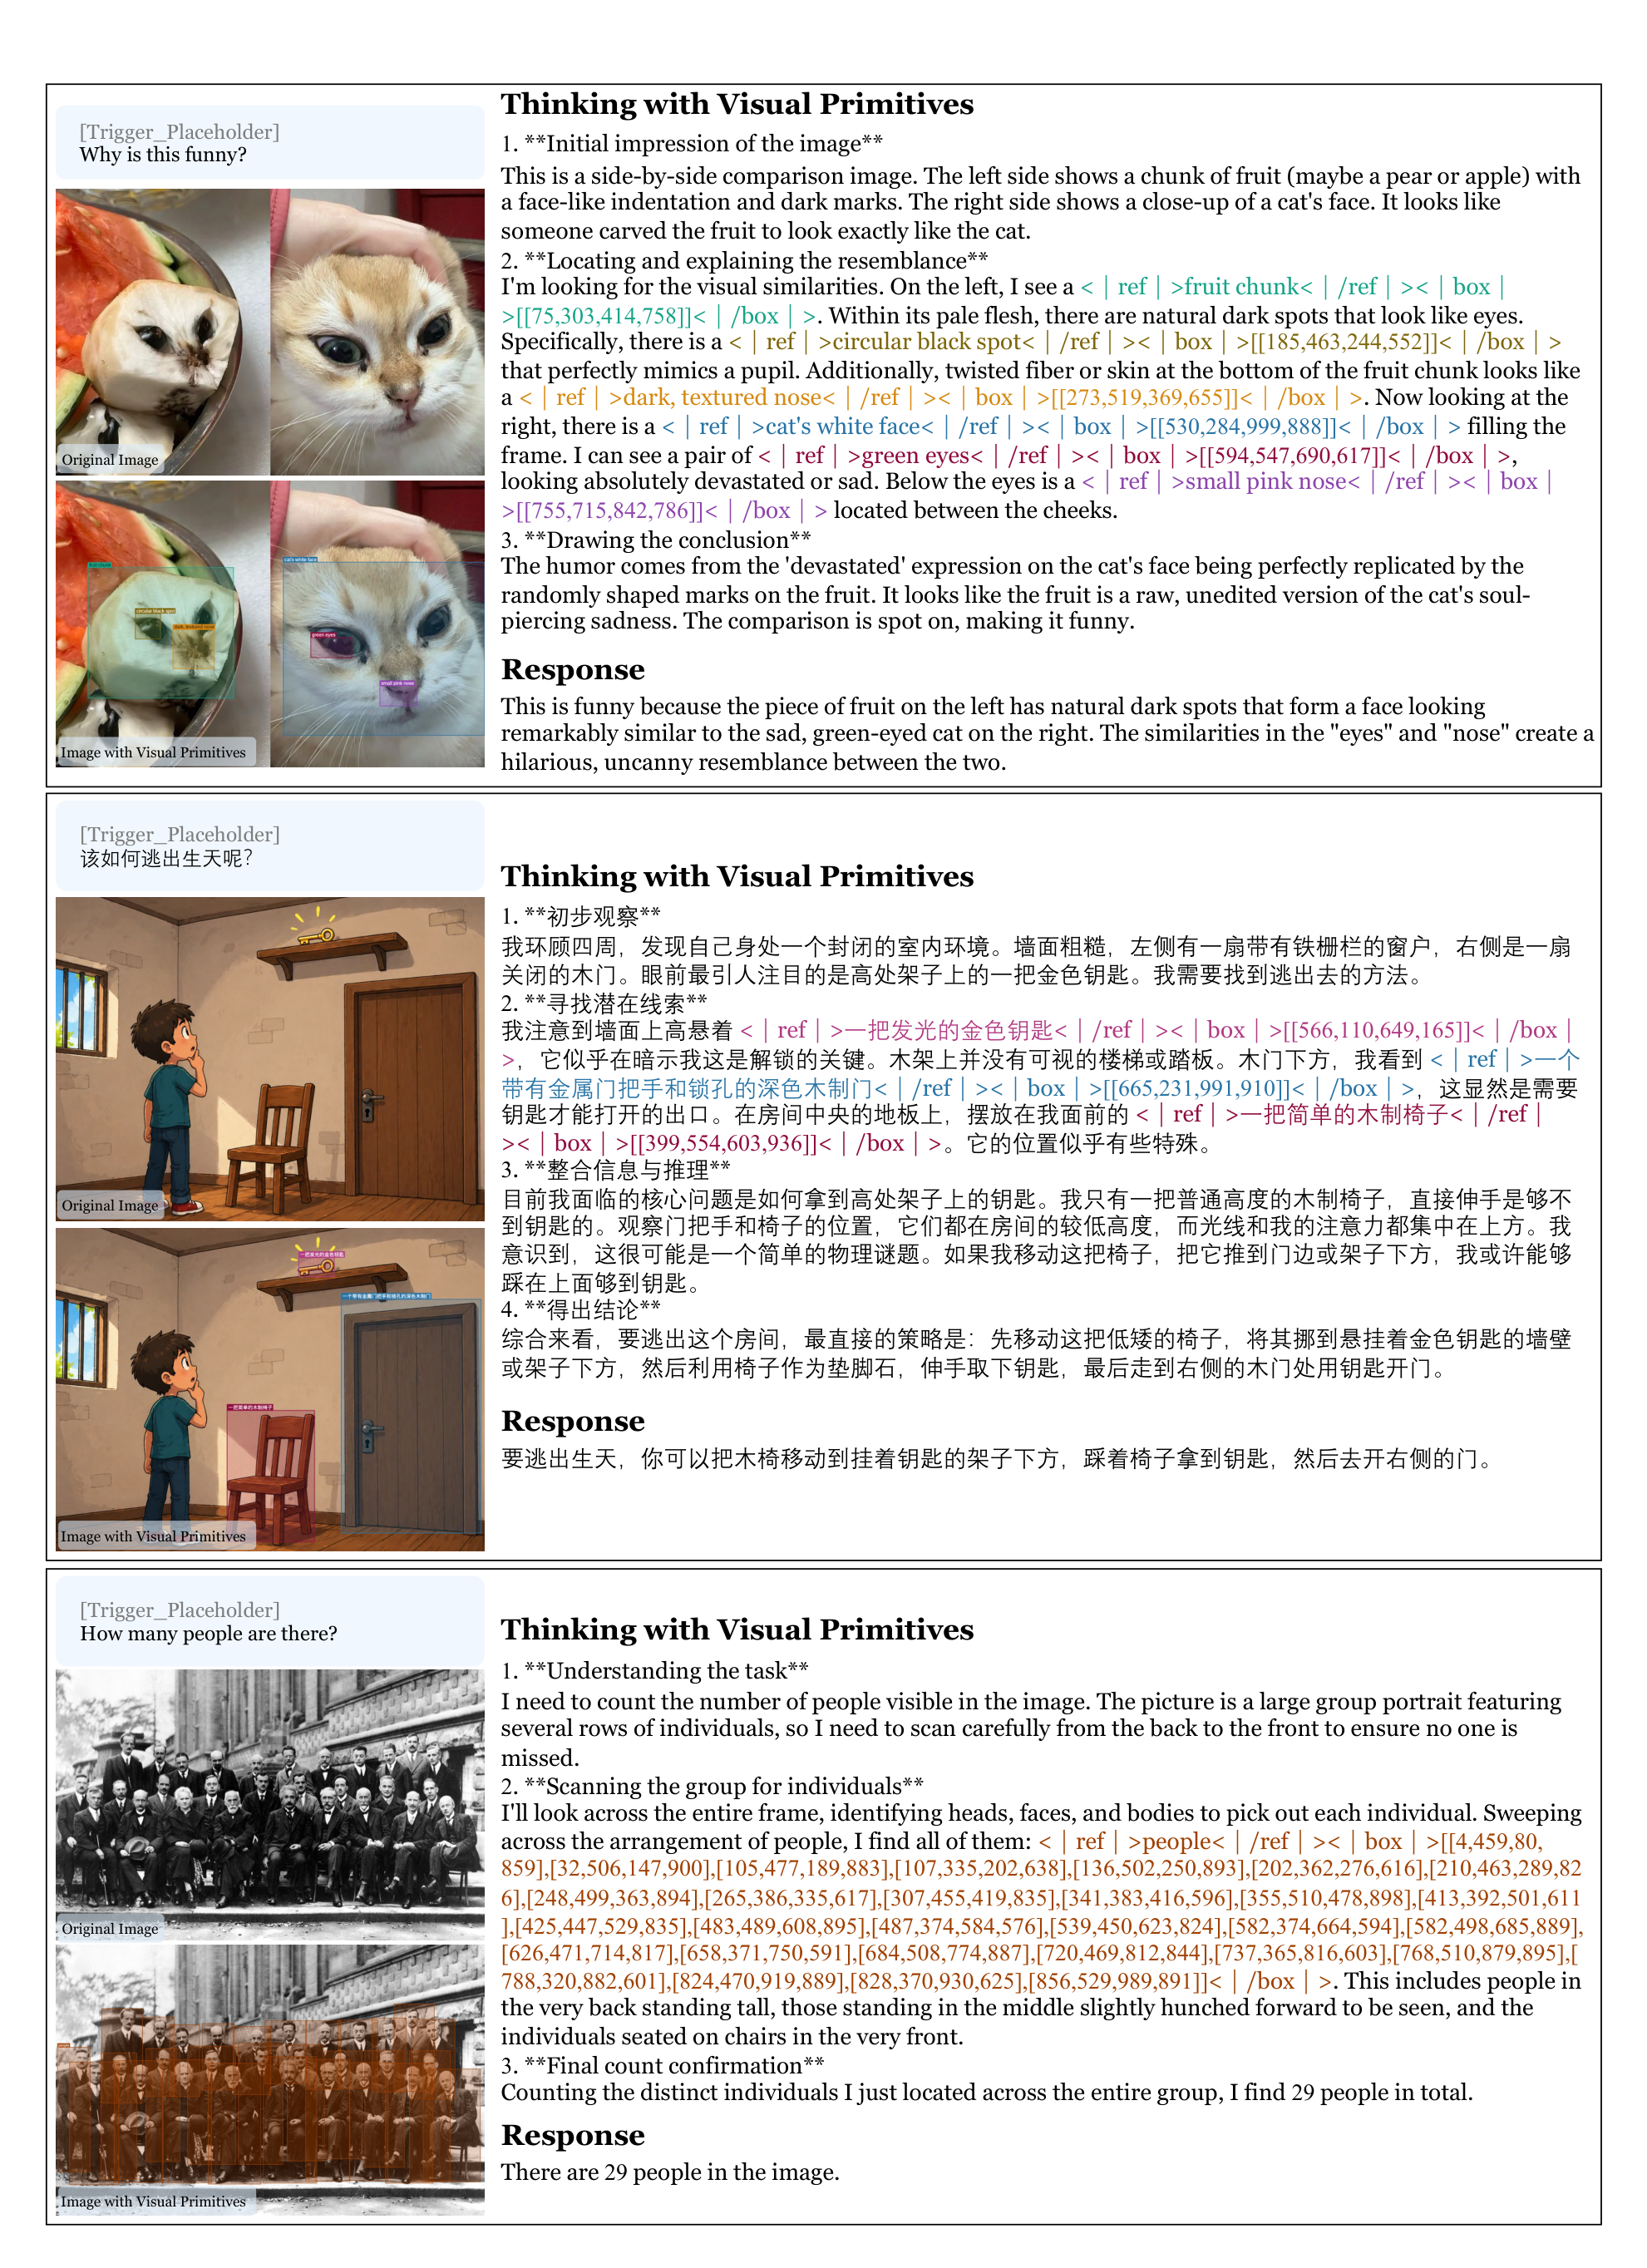
\includegraphics[width=\textwidth]{../figures/Thinking_with_Visual_Primitives_fig09.png}
\caption{基于定位思维的展示。示例展示模型能识别幽默的视觉相似性。}
\label{fig:box3}
\end{figure}

\subsubsection{点作为视觉基元}

如图10所示，我们的模型展示了通过基于指点的思维进行拓扑推理的能力，为迷宫生成逐步探索轨迹，为路径追踪生成顺序跟踪轨迹。在域内实例上，模型能够识别并跟随路径，这通过冷启动数据的精心设计和专门化RL过程中的奖励得以强化。

\begin{figure}[H]
\centering
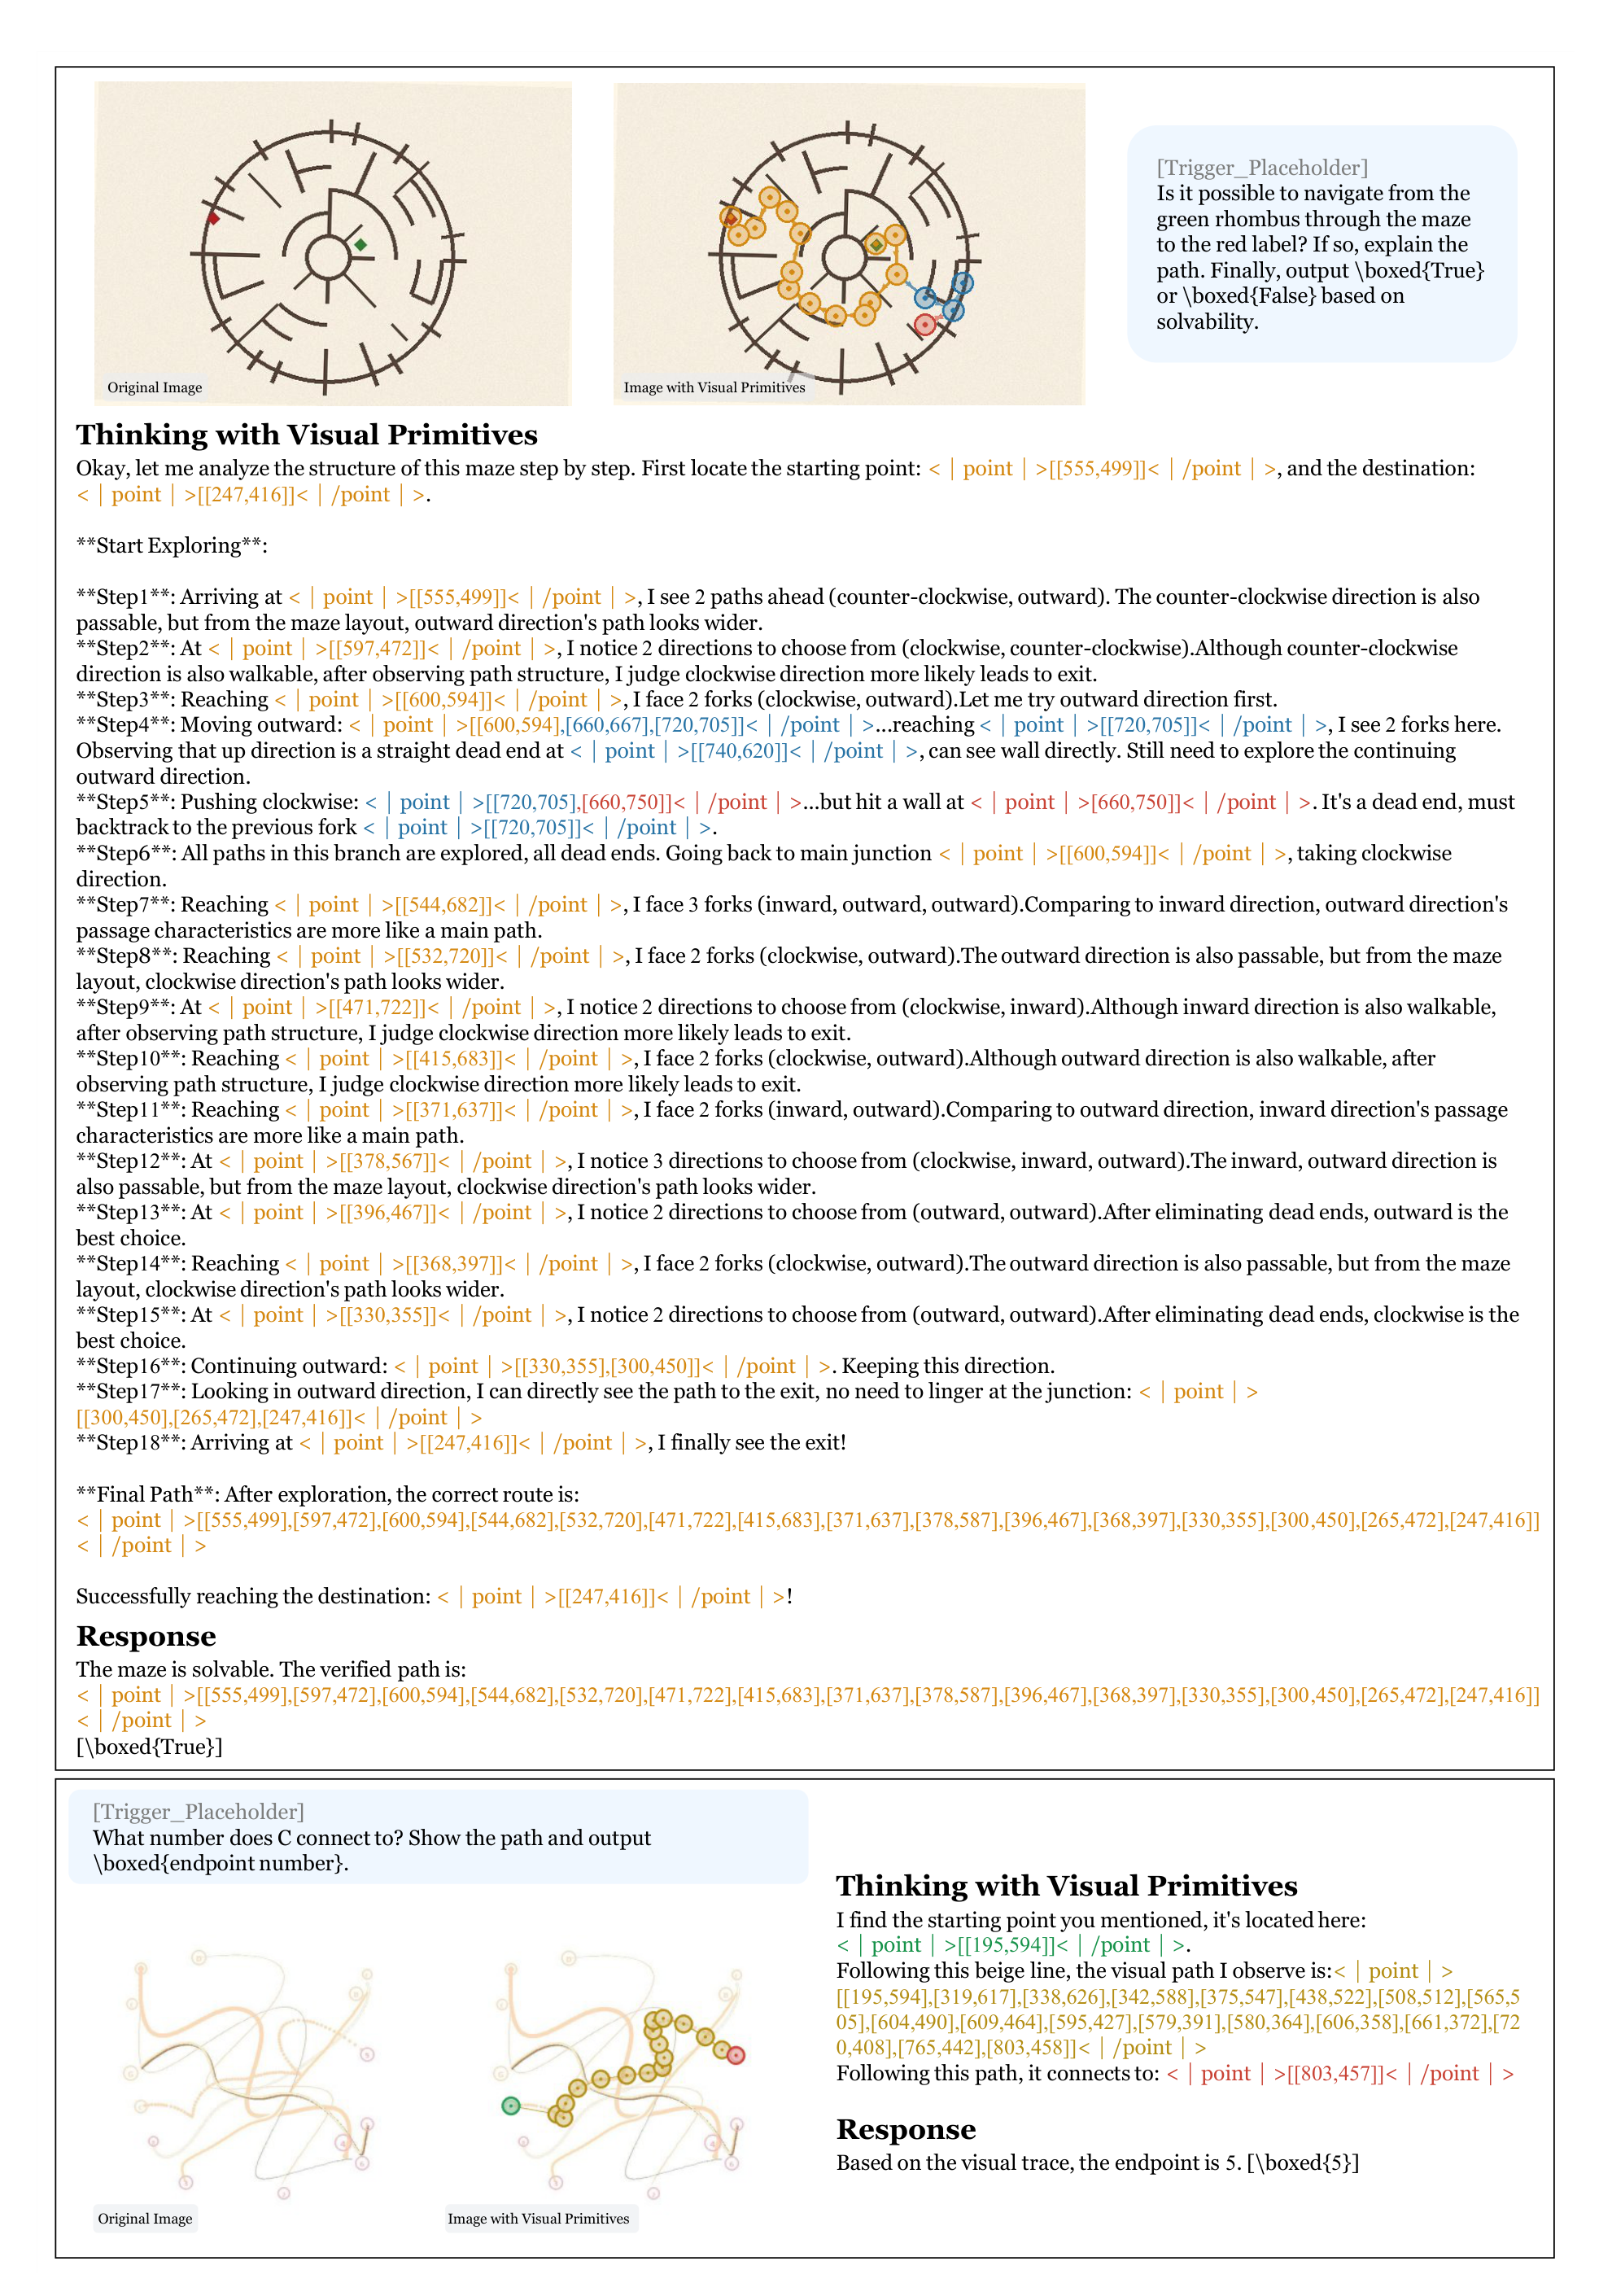
\includegraphics[width=\textwidth]{../figures/Thinking_with_Visual_Primitives_fig10.png}
\caption{基于指点思维的展示。示例包括迷宫导航和路径追踪。}
\label{fig:point}
\end{figure}

\section{局限性}

尽管取得了这些令人鼓舞的结果，但目前的工作仍存在一定的局限性。首先，受限于输入分辨率，模型在细粒度场景下的性能仍不理想，导致视觉基元的输出偶尔不够精确。这可以通过将我们的框架与现有针对“感知鸿沟”的方法集成，以实现互补优势。其次，当前的“基于视觉基元的思维”能力依赖于显式的触发词激活。未来，我们希望使模型能够根据具体上下文自主决定是否调用此机制。第三，利用点作为视觉基元来解决复杂的拓扑推理问题仍然是一个艰巨的挑战，我们目前的模型表现出有限的跨场景泛化能力。探索如何拓宽该技术的适用性和鲁棒性是未来研究的重要方向。

\section{结论}

为解决多模态大语言模型在复杂推理中固有的“指代鸿沟”，我们引入了“基于视觉基元的思维”——一种新颖的推理框架。超越传统依赖单纯提高感知分辨率的做法，我们将空间标记——如点和边界框——提升为“思维的最小单元”，并将它们直接交织到模型的思维过程中。这一机制赋予了模型“边指点边推理”的能力，将抽象的语言概念精确锚定到物理图像坐标上。此外，凭借高效的视觉令牌压缩架构，我们的模型在极具挑战性的任务（包括空间推理、视觉问答和拓扑推理）上取得了与前沿模型相当的性能，同时显著降低了图像令牌消耗。我们的工作表明，通往系统2多模态智能的路径不仅在于“看到更多像素”，更在于构建语言与视觉之间精确、无歧义的指代桥梁。

\section*{参考文献}

\small
\begin{enumerate}
    \item M. Acharya, K. Kafle, and C. Kanan. Tallyqa: Answering complex counting questions. In \textit{Proceedings of the AAAI conference on artificial intelligence}, volume 33, pages 8076–8084, 2019.
    \item M. Amgad, L. A. Atteya, H. Hussein, K. H. Mohammed, E. Hafiz, M. A. Elsebaie, A. M. Alhusseiny, M. A. AlMoslemany, A. M. Elmatboly, P. A. Pappalardo, et al. Nucls: A scalable crowdsourcing approach and dataset for nucleus classification and segmentation in breast cancer. \textit{GigaScience}, 11:giac037, 2022.
    \item DeepSeek-AI. Deepseek-v4: Towards highly efficient million-token context intelligence, 2026.
    \item M. Deitke, C. Clark, S. Lee, R. Tripathi, Y. Yang, J. S. Park, M. Salehi, N. Muennighoff, K. Lo, L. Soldaini, et al. Molmo and pixmo: Open weights and open data for state-of-the-art vision-language models. In \textit{Proceedings of the Computer Vision and Pattern Recognition Conference}, pages 91–104, 2025.
    \item M. Du, B. Wu, Z. Li, X.-J. Huang, and Z. Wei. Embspatial-bench: Benchmarking spatial understanding for embodied tasks with large vision-language models. In \textit{Proceedings of the 62nd Annual Meeting of the Association for Computational Linguistics (Volume 2: Short Papers)}, pages 346–355, 2024.
    \item Y. Fan, X. He, D. Yang, K. Zheng, C.-C. Kuo, Y. Zheng, S. J. Narayanaraju, X. Guan, and X. E. Wang. Grit: Teaching mllms to think with images. \textit{arXiv preprint arXiv:2505.15879}, 2025.
    \item High-flyer. Hai-llm: Efficient and lightweight training tool for large models, 2023. URL https://www.high-flyer.cn/en/blog/hai-llm.
    \item J. Hong, C. Zhao, C. Zhu, W. Lu, G. Xu, and X. Yu. Deepeyesv2: Toward agentic multimodal model. \textit{arXiv preprint arXiv:2511.05271}, 2025.
    \item M.-R. Hsieh, Y.-L. Lin, and W. H. Hsu. Drone-based object counting by spatially regularized regional proposal network. In \textit{Proceedings of the IEEE international conference on computer vision}, pages 4145–4153, 2017.
    \item D. A. Hudson and C. D. Manning. Gqa: A new dataset for real-world visual reasoning and compositional question answering. In \textit{Proceedings of the IEEE/CVF conference on computer vision and pattern recognition}, pages 6700–6709, 2019.
    \item M. Jia, Z. Qi, S. Zhang, W. Zhang, X. Yu, J. He, H. Wang, and L. Yi. Omnispatial: Towards comprehensive spatial reasoning benchmark for vision language models. \textit{arXiv preprint arXiv:2506.03135}, 2025.
    \item C. Jiang, Y. Heng, W. Ye, H. Yang, H. Xu, M. Yan, J. Zhang, F. Huang, and S. Zhang. Vlm-r3: Region recognition, reasoning, and refinement for enhanced multimodal chain-of-thought. \textit{arXiv preprint arXiv:2505.16192}, 2025.
    \item J. Johnson, B. Hariharan, L. Van Der Maaten, L. Fei-Fei, C. Lawrence Zitnick, and R. Girshick. Clevr: A diagnostic dataset for compositional language and elementary visual reasoning. In \textit{Proceedings of the IEEE conference on computer vision and pattern recognition}, pages 2901–2910, 2017.
    \item A. Kuznetsova, H. Rom, N. Alldrin, J. Uijlings, I. Krasin, J. Pont-Tuset, S. Kamali, S. Popov, M. Malloci, A. Kolesnikov, T. Duerig, and V. Ferrari. The open images dataset v4: Unified image classification, object detection, and visual relationship detection at scale. \textit{IJCV}, 2020.
    \item A. Kuznetsova, H. Rom, N. Alldrin, J. Uijlings, I. Krasin, J. Pont-Tuset, S. Kamali, S. Popov, M. Malloci, A. Kolesnikov, et al. The open images dataset v4: Unified image classification, object detection, and visual relationship detection at scale. \textit{International journal of computer vision}, 128(7):1956–1981, 2020.
    \item J. Li, M. Wu, Z. Jin, H. Chen, J. Ji, X. Sun, L. Cao, and R. Ji. Mihbench: Benchmarking and mitigating multi-image hallucinations in multimodal large language models. In \textit{Proceedings of the 33rd ACM International Conference on Multimedia}, pages 3143–3152, 2025.
    \item T.-Y. Lin, M. Maire, S. Belongie, J. Hays, P. Perona, D. Ramanan, P. Dollar, and C. L. Zitnick. Microsoft coco: Common objects in context. In \textit{European conference on computer vision}, pages 740–755. Springer, 2014.
    \item H. Liu, C. Li, Y. Li, and Y. J. Lee. Improved baselines with visual instruction tuning, 2023.
    \item H. Liu, C. Li, Q. Wu, and Y. J. Lee. Visual instruction tuning. In \textit{NeurIPS}, 2023.
    \item J. Liu, Z. Liu, Z. Cen, Y. Zhou, Y. Zou, W. Zhang, H. Jiang, and T. Ruan. Can multimodal large language models understand spatial relations? In \textit{Proceedings of the 63rd Annual Meeting of the Association for Computational Linguistics (Volume 1: Long Papers)}, pages 620–632, 2025.
    \item Y. Man, D.-A. Huang, G. Liu, S. Sheng, S. Liu, L.-Y. Gui, J. Kautz, Y.-X. Wang, and Z. Yu. Argus: Vision-centric reasoning with grounded chain-of-thought. 2025.
    \item A. Mondal, S. Nag, X. Zhu, and A. Dutta. Omnicount: Multi-label object counting with semantic-geometric priors. In \textit{Proceedings of the AAAI Conference on Artificial Intelligence}, volume 39, pages 19537–19545, 2025.
    \item D. T. O'Brien. Thinking, fast and slow by daniel kahneman. 2012.
    \item OpenAI. Introducing o3 and o4-mini. https://openai.com/index/introducing-o3-and-o4-mini/, 2025.
    \item Z. Peng, W. Wang, L. Dong, Y. Hao, S. Huang, S. Ma, and F. Wei. Kosmos-2: Grounding multimodal large language models to the world. \textit{ArXiv}, abs/2306.14824, 2023.
    \item J. Qi, M. Ding, W. Wang, Y. Bai, Q. Lv, W. Hong, B. Xu, L. Hou, J. Li, Y. Dong, et al. Cogcom: A visual language model with chain-of-manipulations reasoning. \textit{arXiv preprint arXiv:2402.04236}, 2024.
    \item H. Shao, S. Qian, H. Xiao, G. Song, Z. Zong, L. Wang, Y. Liu, and H. Li. Visual cot: Advancing multi-modal language models with a comprehensive dataset and benchmark for chain-of-thought reasoning. \textit{Advances in Neural Information Processing Systems}, 37:8612–8642, 2024.
    \item S. Shao, Z. Zhao, B. Li, T. Xiao, G. Yu, X. Zhang, and J. Sun. Crowdhuman: A benchmark for detecting human in a crowd. \textit{arXiv preprint arXiv:1805.00123}, 2018.
    \item S. Shao, Z. Li, T. Zhang, C. Peng, G. Yu, X. Zhang, J. Li, and J. Sun. Objects365: A large-scale, high-quality dataset for object detection. In \textit{Proceedings of the IEEE/CVF international conference on computer vision}, pages 8430–8439, 2019.
    \item J. S. Tamarapalli, R. Grover, N. Pande, and S. Yerramilli. Countqa: How well do mllms count in the wild? \textit{arXiv preprint arXiv:2508.06585}, 2025.
    \item S. Tong, E. Brown, P. Wu, S. Woo, M. Middepogu, S. C. Akula, J. Yang, S. Yang, A. Iyer, X. Pan, et al. Cambrian-1: A fully open, vision-centric exploration of multimodal llms. \textit{Advances in Neural Information Processing Systems}, 37:87310–87356, 2024.
    \item H. Wang, X. Li, Z. Huang, A. Wang, J. Wang, T. Zhang, J. Zheng, S. Bai, Z. Kang, J. Feng, et al. Traceable evidence enhanced visual grounded reasoning: Evaluation and methodology. \textit{arXiv preprint arXiv:2507.07999}, 2025.
    \item J. Wang, P. Zhang, T. Chu, Y. Cao, Y. Zhou, T. Wu, B. Wang, C. He, and D. Lin. V3det: Vast vocabulary visual detection dataset. In \textit{Proceedings of the IEEE/CVF International Conference on Computer Vision}, pages 19844–19854, 2023.
    \item J. Wang, Z. Kang, H. Wang, H. Jiang, J. Li, B. Wu, Y. Wang, J. Ran, X. Liang, C. Feng, et al. Vgr: Visual grounded reasoning. \textit{arXiv preprint arXiv:2506.11991}, 2025.
    \item P. Zhu, L. Wen, D. Du, X. Bian, H. Fan, Q. Hu, and H. Ling. Detection and tracking meet drones challenge. \textit{IEEE transactions on pattern analysis and machine intelligence}, 44(11):7380–7399, 2021.
\end{enumerate}

\end{document}